\documentclass[
    11pt,
    a4paper,
    egregdoesnotlikesansseriftitles,
    toc=chapterentrywithdots,
    oneside,openright,
    titlepage,
    parskip=half,
    headings=normal,  % reduces heading size
    listof=totoc,
    bibliography=totoc,
    index=totoc,
	captions=tableheading,  % caption below table
%    chapterprefix,
    listof=flat,
    final
]{scrbook}


% details about your thesis
\newcommand{\titel}{Betrachtung aktueller Chancen von Progressive Web Apps im Gegensatz zu Native Apps}
\newcommand{\artderarbeit}{Bachelorarbeit}  % {Bachelorarbeit,Masterarbeit}
\newcommand{\autor}{Mahja Sarschar}
\newcommand{\studiengang}{Medieninformatik}  % {Informatik,Wirtschaftsinformatik,Medieninformatik}
\newcommand{\matrikelnr}{320\,1818}
\newcommand{\erstgutachter}{Prof.\,Dr.~Matthias\,Teßmann}
\newcommand{\zweitgutachter}{Prof.\,Dr.~Christian\,Schiedermeier}
\newcommand{\betreuer}{Dipl.-Ing.\,~Michael\,Müller}
\newcommand{\unternehmen}{OPITZ\,CONSULTING\,GmbH}
\newcommand{\logo}{figures/TH-Nuernberg-RGB.png}
\newcommand{\keywords}{progressive web app, native apps, html5} 

% custom head and foot
\usepackage[automark]{scrlayer-scrpage}
\pagestyle{scrheadings}
\ihead{\headmark}
\chead{}
\ohead{\pagemark}
\renewcommand*\chaptermarkformat{\chapappifchapterprefix{\ }% 
  \thechapter.\enskip}

\RedeclareSectionCommand[tocindent=0pt]{section}
\RedeclareSectionCommand[tocindent=0pt]{subsection}
%\RedeclareSectionCommand[tocnumwidth=70pt]{chapter}

\usepackage{scrhack}

% other packages
\usepackage[utf8]{inputenc}
\usepackage[T1]{fontenc}
\usepackage{lmodern,relsize,textcomp,csquotes}
\usepackage{amsmath,amsfonts}
\usepackage[ngerman]{babel}  % flip for German thesis
\usepackage[final]{graphicx}
\usepackage{setspace,geometry,xcolor}
\usepackage{makeidx}
\usepackage{paralist,ifthen,todonotes}
\usepackage{url}
\usepackage[toc]{glossaries}
\usepackage{pdfpages}
\usepackage{subfigure}
\usepackage{acronym}
\usepackage{makecell}
\usepackage{multirow}

% table setup
\usepackage{longtable}
\usepackage{array}
\usepackage{ragged2e}
\usepackage{lscape}

% pdf hyperref
\usepackage[
    bookmarks=true,
    bookmarksopen=true,
    bookmarksnumbered=true,
    bookmarksopenlevel=1,
    pdftitle={\titel},
    pdfauthor={\autor},
    pdfcreator={\autor},
    pdfsubject={\titel},
    pdfkeywords={\keywords},
    pdfpagelabels=true,
    colorlinks=true,
    linkcolor=black,
    urlcolor=black,
    anchorcolor=black,
    citecolor=black,
    filecolor=black,
    menucolor=black,
    plainpages=false,
    hypertexnames=true,
    linktocpage=true,
]{hyperref}


% configure your listings style
\usepackage{listings}
\lstset{
	tabsize=3,
	extendedchars=true,
	frame=single,
	showstringspaces=false,
	numbers=left,
	numberstyle=\small,
	breakautoindent=true
}

% page setup
% \setlength{\topskip}{\ht\strutbox}
\geometry{paper=a4paper,left=2.5cm,top=3.0cm,bindingoffset=.8cm}
\onehalfspacing
\frenchspacing
\clubpenalty = 10000
\widowpenalty = 10000 
\displaywidowpenalty = 10000

% some commands
\newcommand{\ua}{\mbox{u.\,a.\ }}
\newcommand{\zB}{\mbox{z.\,B.\ }}
\newcommand{\dahe}{\mbox{d.\,h.,\ }}
\newcommand{\bzw}{\mbox{bzw.\ }}
\newcommand{\bzgl}{\mbox{bzgl.\ }}
\newcommand{\kA}{\mbox{k. A.\ }}
\newcommand{\wrt}{\mbox{w.\,r.\,t.\ }}
\newcommand{\etal}{\mbox{\emph{et.\,al.\ }}}
\newcommand*{\quelle}[1]{\par\raggedleft\footnotesize Quelle:~#1}

%acronym plurals
\acrodefplural{pwa}[PWAs]{Progressive Web Apps}
\acrodefplural{sdk}[SDKs]{Software development kits}
\acrodefplural{spa}[SPAs]{Single-Page Applications}
\acrodefplural{api}[APIs]{Application Programming Interfaces}

% load glossary entries
%\makenoidxglossaries
%\loadglsentries{glossary}

\begin{document}

\setcounter{secnumdepth}{3}  % numerate subsections
\setcounter{tocdepth}{2}  % ...but don't include them in toc

\frontmatter
\thispagestyle{empty}
\pdfbookmark[1]{Cover}{cov}
\begin{titlepage}

\begin{center}

\includegraphics[width=\linewidth]{figures/TH-Nuernberg-RGB.png}\\[1cm]
\LARGE{Fakultät Informatik}\\[1cm]

\huge
\textbf{\titel}\\[1cm]
%
\Large
\artderarbeit~im Studiengang \studiengang\\[1cm]
%
\large
vorgelegt von

\Large
\autor\\[0.5cm]
\small
Matrikelnummer \matrikelnr\\[1cm]
%\vspace*{\fill}
\large
\begin{tabular}{p{3cm}p{8cm}}\\
Erstgutachter:  & \quad \erstgutachter\\[1.2ex]
Zweitgutachter: & \quad \zweitgutachter\\[1.2ex]
Betreuer: & \quad \betreuer\\
Unternehmen: & \quad \unternehmen
\end{tabular}
\singlespacing

\includegraphics[height=1.5cm]{figures/OC-Logo RGB.png} 
\singlespacing
\copyright\,\the\year
\end{center}
\vspace{-0.5cm}
\singlespacing
\small
\noindent Dieses Werk einschließlich seiner Teile ist \textbf{urheberrechtlich geschützt}.
Jede Verwertung außerhalb der engen Grenzen des Urheberrechtgesetzes ist ohne Zustimmung des Autors unzulässig und strafbar.
Das gilt insbesondere für Vervielfältigungen, Übersetzungen, Mikroverfilmungen sowie die Einspeicherung und Verarbeitung in elektronischen Systemen.

\end{titlepage}\cleardoublepage

% download the following form and complete it (hit save in your editor)
% https://intern.ohmportal.de/fileadmin/Gelenkte_Doks/Abt/SZS/SB/SB_0050_FO_Pruefungsrechtliche_Erklaerung_und_Erklaerung_zur_Veroeffentlichung_der_Abschlussarbeit_public.pdf
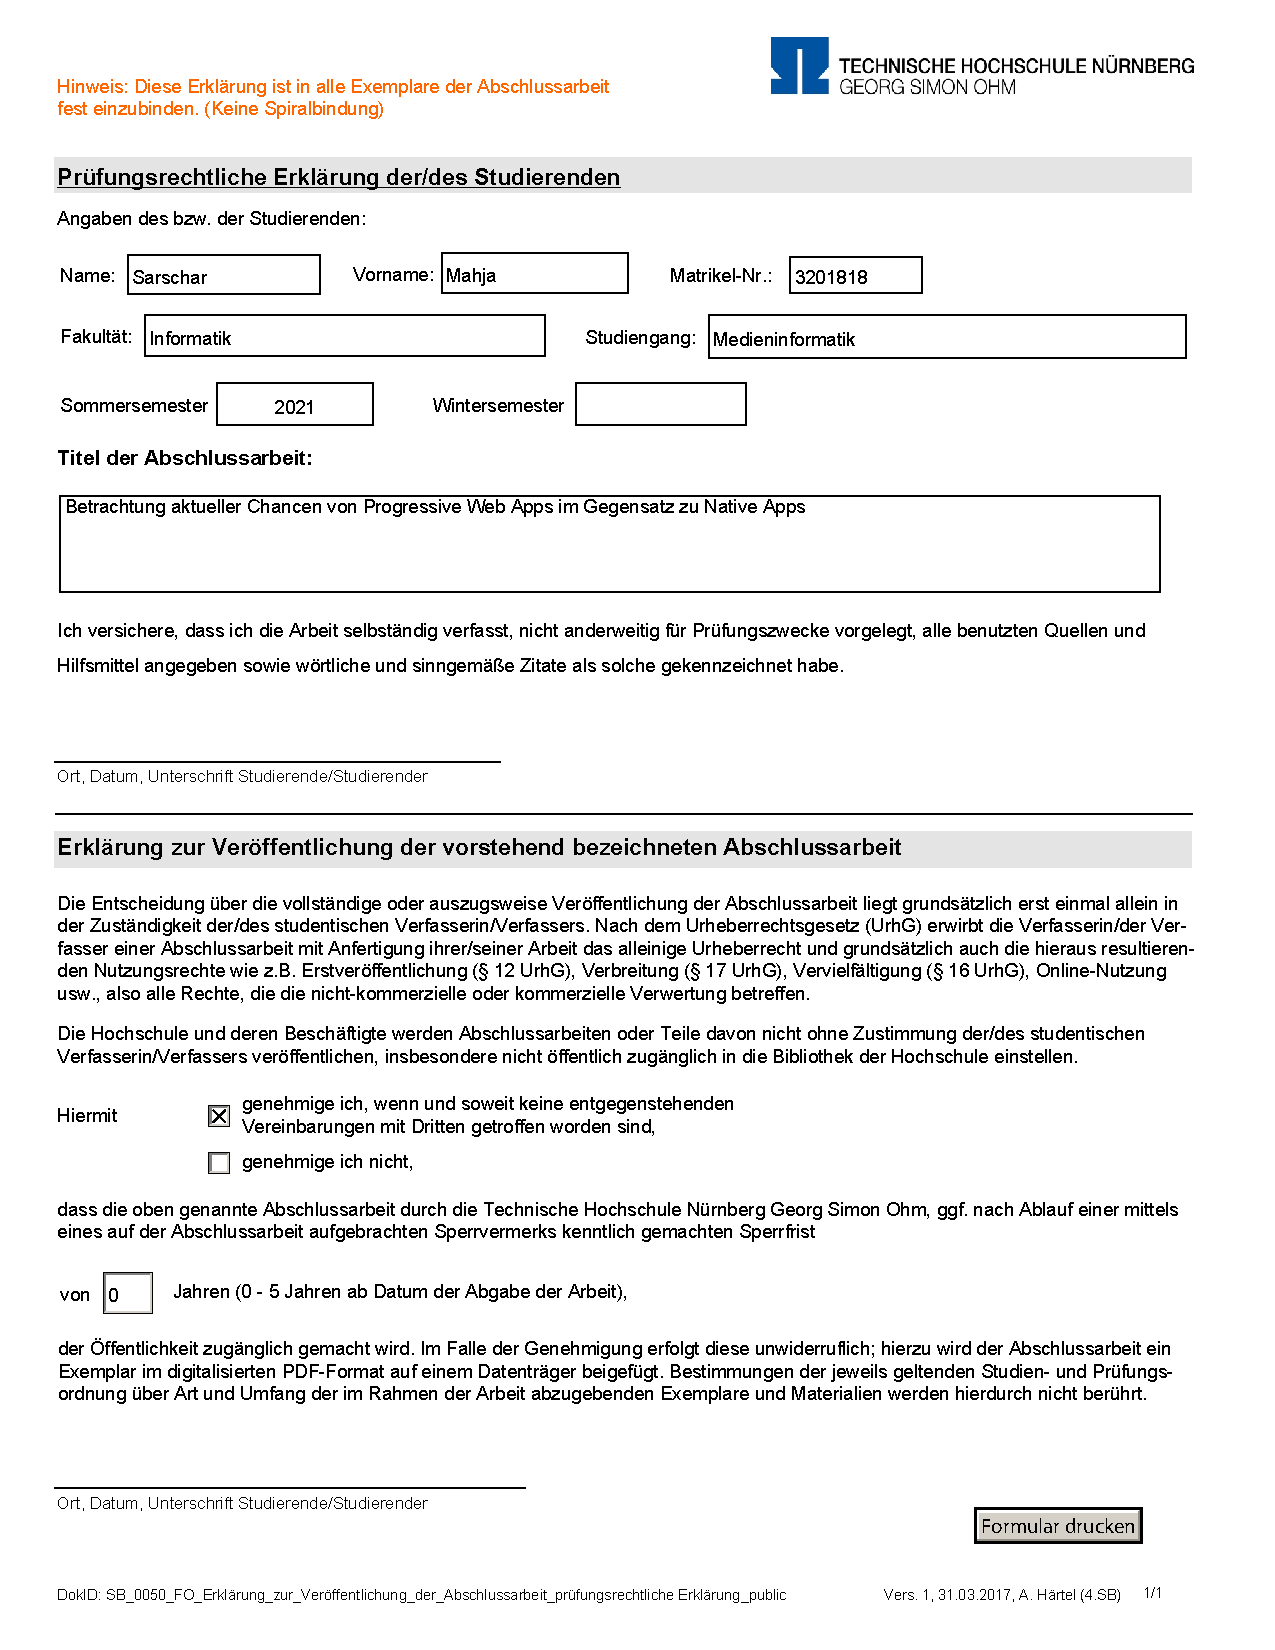
\includepdf{SB_0050_FO_Pruefungsrechtliche_Erklaerung_und_Erklaerung_zur_Veroeffentlichung_der_Abschlussarbeit_public.pdf}

\thispagestyle{empty}
\section*{Kurzdarstellung}
\label{sec:kurzdarstellung}
%Warum ist es wichtig das jetzt zu machen?
%Worum geht es?
%Wie bist du vorgegangen?
%Was sind deine wichtigsten Ergebnisse?
%Was bedeuten deine Ergebnisse?
In der vorliegenden Bachelorarbeit wird untersucht, ob und welche Vor- und Nachteile das Entwickeln einer Progressive Web App -- eine Webanwendung, die Funktionalitäten wie Offlinebetrieb und Installation unterstützt -- im Gegensatz zu einer nativen Anwendung bieten. 
Ferner soll damit die Frage beantwortet werden, ob sie diese ersetzen kann, um die Chancen von Progressive Web Apps zu analysieren.
Die Besonderheit dabei ist, dass für die Entwicklung der Native App ein plattformunabhängiger Ansatz gewählt wurde, um die Technologien auf eine vergleichbare Ebene zu bringen.\\
Für den Vergleich wurde auf Basis eines Kriterienkatalogs, bestehend aus Funktionalität, Kompatibilität mit verschiedenen Betriebssystemen und Entwicklungsaufwand, jeweils eine App entwickelt.
Diese stellt die aktuellen COVID-19 Fallzahlen dar und unterstützt neben dem Offlinebetrieb und der Installation die Funktionen Standortzugriff, Kontaktzugriff und Benachrichtigungen.\\
Bei den implementierten Funktionalitäten wird deutlich, dass Progressive Web Apps mittlerweile durch eine Vielzahl von modernen Schnittstellen des Webs eine Alternative zu Native Apps darstellen können.
Dabei ist jedoch eine Schwachstelle von Progressive Web Apps die fehlende Unterstützung einiger Funktionalitäten von iOS.
Der Entwicklungsaufwand einer Progressive Web App ist geringer als der einer Native App.\\
Zusammenfassend zeigt das Ergebnis, dass Progressive Web Apps das Potential besitzen, native Anwendungen zu ersetzen.
Aktuell ist die Technologie jedoch nicht ausreichend ausgereift, dass sie jegliche native Anwendung ersetzen kann und muss somit abhängig von den Anforderungen des Anwendungsfalls betrachtet werden.\cleardoublepage

\tableofcontents

\listoffigures
\cleardoublepage

\listoftables
\cleardoublepage

\renewcommand{\lstlistlistingname}{Listings}  % change for German thesis
\lstlistoflistings
\cleardoublepage

\chapter*{Abkürzungsverzeichnis}
\begin{acronym}
\acro{apk}[APK]{Android Package}
\acro{api}[API]{Application Programming Interface}
\acro{apn}[APNs]{Apple Push Notification service}
\acro{avd}[AVD]{Android Virtual Device}
\acro{cdn}[CDN]{Continous Delivery Network}
\acro{dom}[DOM]{Document Object Model}
\acro{fcm}[FCM]{Firebase Cloud Messaging}
\acro{gps}[GPS]{Global Positioning System}
\acro{https}[HTTPS]{Hypertext Transfer Protocol Secure}
\acro{ide}[IDE]{Integrated development environment}
\acro{ipa}[ipa]{iOS App Store Package}
\acro{json}[JSON]{JavaScript Object Notation}
\acro{pwa}[PWA]{Progressive Web App}
\acro{spa}[SPA]{Single-Page Application}
\acro{sdk}[SDK]{Software Development Kit}
\acro{ui}[UI]{User Interface}
\acro{url}[URL]{Uniform Resource Locator}
\end{acronym}
\cleardoublepage

\mainmatter
\chapter{Einleitung}\label{ch:intro}
%Thema einleiten: Ich vergleiche PWAs mit nativen Apps.
%erklären was native ist und was da so geht
Egal ob Spotify, TikTok oder Twitter - mobilen Anwendungen sind aus unserem Lebensalltag nicht mehr wegzudenken.
Dafür sprechen auch die stetig zunehmende Anzahl an App Downloads, welche 2020 bei 218 Billionen liegt \cite{Iqbal.06.05.2021}.\\
Bei der Entwicklung dieser Anwendungen gibt es jedoch immer wieder auftretende Problematiken.
Beispielsweise die fehlende Kompatibilität einer plattformspezifischen App mit verschiedenen Betriebssystemen und der daraus folgende erhöhte Entwicklungsaufwand.
Außerdem muss der Nutzer erst überzeugt werden, die Anwendung zu installieren, bevor er sie überhaupt nutzen kann.

%% warum ist pwas besser als native? --> überleitung
Ein aufstrebendes Konzept, dass sich die Universalität des Webs zu nutzen macht, ist das der \acp{pwa}.
Diese besonderen Anwendungen sind über das Web erreichbar und sollen die Freiheiten einer Browseranwendung mit den Vorzügen einer nativen Applikation vereinen.
2015 von dem Chrome Entwickler Alex Russel und dem Designer Frances Berriman als solche benannt, bieten \acp{pwa} immer mehr Möglichkeiten an \cite{Russell.2015}.
Dabei spielt auch die Weiterentwicklung von Webschnittstellen eine bedeutsame Rolle.
Mit Technologien wie den Service Worker und dem App Manifest ermöglichen PWAs Funktionalitäten, die bislang nativen Anwendungen vorenthalten waren.
Dazu gehören beispielsweise Push Benachrichtigungen, Standortzugriff, Offlinebetrieb und Installierbarkeit.

Gerade in der aktuellen Zeit, in der laut einer Statistik von \textit{StatCounter} 4,32 Billionen Menschen das Internet von mobilen Endgeräten aus nutzen, bietet sich somit eine enorme Chance für die Zukunft von mobilen Anwendungen und des Webs \cite{StatCounter.2021}.
Daher ist der Vergleich von \acp{pwa} mit einer Nativen App relevant und wird in der vorliegenden Arbeit untersucht.

\section{Zielsetzung}
%Warum wurde diese Arbeit mit genau dieser Zielsetzung bearbeitet?
%fachliche Kontext und die Relevanz der Fragestellung  werden nicht sichtbar
Im Rahmen dieser Arbeit soll untersucht werden, welche Vor- und Nachteile das Entwickeln einer \ac{pwa} gegenüber einer nativen App bezüglich Funktionalität, Kompatibilität mit verschiedenen Betriebssystemen und Entwicklungsaufwand bietet.
Um beide Verfahren vergleichen zu können, wird für die Entwicklung der Native App das Framework React Native verwendet, da dies - ähnlich zu \acp{pwa} - plattformunabhängig ist.
Diese Besonderheit wurde bisher noch nicht betrachtet. %?
%Die Besonderheit stellt dabei die Entwicklung einer nativen App mit React Native dar, da dies den Vorteil von Plattformunabhängigkeit aufweist, im Gegensatz zu der nativen Entwicklung von Apps.
Außerdem sollen dabei auch die aktuellen Grenzen von \acp{pwa} aufgezeigt und somit die Frage beantwortet werden, ob \acp{pwa} Native Apps zum jetzigen Zeitpunkt ersetzen können.

\section{Umfeld}
Das Thema der Arbeit wird in Zusammenarbeit mit dem IT-Consulting Unternehmen OPITZ CONSULTING bearbeitet.
Die Betreuung findet durch Senior Consultant Michael Müller statt.
Das Unternehmen entwickelt Lösungen für seine Kunden in den Bereichen Applications, Analytics, Infrastructure und Integration.
Da sich die Software- und Webentwicklungsbranche rasant verändert und weiterentwickelt, ist es für die Firma unerlässlich, neue Technologien und Innovationen zu erkennen.
Daraufhin kann Wissen in diesen Bereichen aufgebaut werden, um Lösungen mit diese Technologien potenziellen Kunden anzubieten.
Besonders interessant sind hierbei diejenigen Innovationen, die mit geringem Aufwand eine Vielzahl an Vorteilen mit sich bringen.

\section{Aufbau der Arbeit}
Zuerst soll auf die Grundlagen von mobilen Anwendungen und \acp{pwa} sowie der JavaScript-Bibliothek React und dem Framework React Native eingegangen werden.
Im dritten Kapitel wird ein Kriterienkatalog festgelegt, anhand dessen die implementierten Anwendungen später beurteilt werden.
Dieser soll die Funktionalität, die Kompatibilität mit verschiedenen Betriebssystemen und den Entwicklungsaufwand in Abhängigkeit der verwendeten Technologie berücksichtigen.
Im Anschluss wird die Programmierung der zwei Applikationen vorgestellt und auf spezielle Vorgehensweisen eingegangen.
Der Zweck der Apps ist es, die aktuellen COVID-19 Fallzahlen der offiziellen Datenbank des Robert-Koch-Instituts darzustellen und weiterführende Funktionalitäten wie Installation, Offlinebetrieb, Standortzugriff, Kontaktzugriff und Benachrichtigungen zu unterstützen.
Zuletzt sollen die zwei Anwendungen anhand des Kriterienkatalogs verglichen und bewertet werden.
%Dem Unternehmen soll durch die Ergebnisse der Arbeit ermöglicht werden, für konkrete Anwendungsfällen abwägen zu können, welche der beiden Ansätze sich für die Umsetzung anbietet.
\chapter{Grundlagen}\label{ch:basics}
In diesem Kapitel werden die für diese Arbeit notwendigen Grundlagen aufgezeigt.
Diese sollen für ein einheitliches Verständnis des Themas sorgen und unterschiedliche Vorstellungen von Fachbegriffen angleichen.

Generell lassen sich mobile Anwendungen in drei Kategorien einteilen: Native, Hybrid und Web Applikationen.
Im Folgenden wird einerseits genauer auf Native und Hybride Applikationen und anderseits auf eine spezielle Form von Web Apps, genannt \acp{pwa}, eingegangen.

\section{Native Applikationen}
Als native Applikationen bezeichnet man Anwendungen, die plattformspezifisch -- ergo speziell für ein \ac{os} -- implementiert werden.
Das wird dadurch ermöglicht, dass sie mit dem \ac{sdk} des Plattformherstellers entwickelt werden und somit kompletten Zugriff auf jegliche Funktionalitäten der Geräte besitzen.
Außerdem entsteht durch Verwendung der plattformspezifischen UI-Komponenten\footnote{User Interface Komponenten, z. Dt. Benutzeroberflächenkomponenten}, sogenannten Views, eine einheitliche Benutzerschnittstelle, die sich in allen Anwendungen des Betriebssystems widerspiegelt.
Um solche Apps mit ihren \acp{sdk} zu entwickeln, wird die zur \ac{sdk} zugehörige Programmiersprache verwendet.
Die bekanntesten Programmiersprachen sind Java oder Kotlin für Android Geräte, Objective-C und Swift für iOS. \cite{Jobe.2013}.
Eine aktuelle Statistik von \textit{Statcounter} macht deutlich, dass die am meisten verbreiteten Betriebssysteme Android und iOS sind, weswegen im Verlauf dieser Arbeit ausschließlich auf ebendiese eingegangen wird \cite{o.V..2021b}.

Um Applikationen im jeweiligen App-Store veröffentlichen zu können, müssen diese eindeutig identifizierbar sein.
Das erfolgt durch den Prozess der sogenannten \textit{Signierung}, der ebenfalls plattformabhängig durchgeführt wird.\\
Eine App kann nach der Signierung und Überprüfung nur durch eine Aktualisierung verändert (\zB Update oder Bugfix) werden.
Deshalb folgt auf eine Aktualisierung auch eine erneute Überprüfung und Veröffentlichung der App.\\
%Danach wird die App teilweise manuell überprüft, bevor sie letztendlich im App-Store publiziert wird.
%Wichtig ist hierbei, dass sich die App, nach jener Überprüfung nicht mehr ändern darf.
%Dies ist erst wieder durch eine offizielle Aktualisierung möglich, welche wiederum den Überprüfungsprozess durchlaufen muss.\\
Ferner können Android Apps auch in ihrer Rohfassung auf Android Geräten installiert werden.
Hierfür muss der Entwicklermodus aktiviert und das \ac{apk}\footnote{Plattformspezifische Sammlung von Dateien, die wie Quellcode und Ressourcen für die Installation und Nutzung der App beinhaltet} auf das Endgerät geladen werden.
Das Äquivalent in iOS ist die \ac{ipa}-Datei.

\section{Cross-platform Applikationen}
Unter cross-platform (z.\,Dt. plattformunabhängig) Applikationen versteht man Anwendungen, die auf einer Code-Basis aufbauen und zur Laufzeit zu mehreren Anwendungen für unterschiedliche Endgeräte kompiliert werden.
%Außerdem können sie in herkömmlichen Quelltext-Editoren entwickelt werden, da sie im Gegensatz zu nativen Anwendungen unabhängig von bestimmten Betriebssystemen oder SDKs sind.
Der Vorteil solcher Applikationen ist, dass sie, obwohl sie auf demselben Code basieren, sich komplett den plattformspezifischen Stil anpassen.
Somit verringern sich auch die Entwicklungskosten, die bei Implementierung von jeweils einer Anwendung pro Betriebssystem anfallen würden.
Klar abzugrenzen sind plattformunabhängige Anwendungen von hybriden Anwendungen.
Denn das Endprodukt bei letzterem ist eine Web Applikation, die sich durch eine WebView in einem nativen Container dem Kontext (\zB Betriebssystem, Auflösung) des Geräts, in dem sie aufgerufen wird, anpasst \cite{Schickler.2015}.

Gängige Frameworks zur plattformunabhängigen Entwicklung sind Electron, Ionic und React Native \cite{o.V..2020}.
Diese stellen meist eine begrenzte Anzahl an vorprogrammierten UI-Komponenten und Funktionalitäten zur Verfügung.
Es gibt außerdem eine Vielzahl von Community Lösungen, die für wiederkehrende Anforderungen Lösungen bieten.

\section{Progressive Web Apps}
\acp{pwa} sind in erster Linie Web Applikationen, also Anwendungen, die mit den üblichen Web Technologien wie HTML, CSS und ECMAScript (JavaScript) implementiert sind.
Laut Mozilla Developer Network zeichnen sie sich dadurch aus, dass zusätzlich folgende technische Voraussetzungen erfüllt sind: Sie müssen auf einer sicheren Verbindung aufbauen, eine oder mehrere Service Worker besitzen und über ein App Manifest verfügen \cite{MDNcontributors.}.
Ersteres wird gewährleistet durch eine \ac{https} Verbindung, während Service Worker JavaScript-Skripte sind, die im Hintergrund auf dem Client und unabhängig von der Anwendung selbst ausgeführt werden \cite{Gaunt.}.
Sie sind die wichtigste Komponente hinter den meisten Funktionalitäten, die eine \ac{pwa} bietet, weswegen im Laufe dieses Kapitels genauer auf ebendiese eingegangen wird. Die letzte benötigte Komponente ist das App Manifest.
Dabei handelt es sich um eine \ac{json}\footnote{Programmiersprachen-unabhängiges Datenformat}-Datei, in der Einzelheiten zur Anwendung und deren Installation angegeben werden \cite{MDNcontributors.b}.
Da es sich dabei, trotz der zusätzlichen nativen Funktionalitäten, um eine Web Applikation handelt, lassen sich \ac{pwa} über eine \ac{url} im Browser aufrufen und sind somit zunächst unabhängig von dem Gerät, auf dem sie aufgerufen werden.
Üblicherweise werden \ac{pwa} als \ac{spa} entwickelt.
Das bedeutet, dass die Anwendung aus einem einzigen HTML-Dokument besteht und Inhalte dynamisch geladen werden.
Ein Vorteil davon ist, dass sich dadurch auch die Anzahl der Anfragen des Clients an den Server verringern, da nicht nach jeder Anfrage die Seite komplett neu angefordert werden muss.
Der Nachteil von \ac{spa} ist, dass im Gegensatz zu klassischen Webanwendungen Funktionalitäten wie Deep-Linking und die Navigation durch die Browser-Steuerelemente eigenständig implementiert werden müssen \cite{Wenzel.2020}.
Bislang gibt es keinen offiziell definierten Web Standard für diese spezielle Art von Webanwendung.

Ein bedeutsames Konzept hinter \acp{pwa} ist das \glqq Progressive Enhancement\grqq{}.
Dieses verlangt, dass \acp{pwa} auf allen Endgeräten grundlegend funktionieren sollen, und schrittweise – falls der Browser und das Gerät dies unterstützt – in ihrer Funktionalität erweitert werden können \cite{Richard.}.
Die Prüfung, ob der Browser die Anforderungen erfüllt, findet durch das Window-Objekt statt, dass das aktuelle Browser Fenster repräsentiert.
Dieses enthält unter anderem das \textit{navigator}-Property, dass Informationen über den Browser besitzt und die Unterstützung der Service Worker \ac{api}\footnote{z.Dt. Programmierschnittstelle.} signalisiert.
Dadurch kann wiederum geprüft werden, ob andere Schnittstellen \zB die \textit{Geolocation}\footnote{Eine Schnittstelle zur Bestimmung und Beobachtung des aktuellen Standorts des Nutzers.} in dem aktuellen Browser unterstützt werden.

%Um eine Übersicht darüber zu erlangen, welche Funktionalitäten durch moderne Webschnittstellen zur Verfügung stehen, bietet sich die Webseite \url{https://whatwebcando.today/} an.
%Dort wird übersichtlich dargestellt, welche konkreten Schnittstellen vom Browser, indem die Webseite aufgerufen wird, unterstützt werden und welche nicht.
%Im Bereich \glqq Native Behaviors\grqq{} fehlt nach Ansicht des Autors beim Aufruf der Seite mit Chrome Browser nur noch die \glqq User Idle Detection\grqq{}.

%Bekannte Bespiele für PWAS? Twitter Lite, Trivago, Forbes siehe https://brainhub.eu/library/pwa-vs-native/
Zur Evaluierung von \ac{pwa} bietet sich \textit{Lighthouse} an, ein vorinstallierte DevTools Erweiterung im Google Chrome Browser.
Dort wird per Mausklick ein Testbericht zur aktuellen Anwendung erstellt, in der unter anderem auch Installierbarkeit und \ac{pwa}-Optimierung geprüft werden.
Dabei orientiert es sich an den, von Web.dev\footnote{Eine von Google Developers unterstützte Webseite mit einer Vielzahl von Artikeln zu Webentwicklungstechnologien.} definierten Kernfunktionalitäten von \ac{pwa}, die lauten: \glqq starts fast, stays fast\grqq , \glqq works in any browser\grqq, \glqq responsive to any screen size\grqq, \glqq provides a custom offline page\grqq, und \glqq is installable\grqq.
Ferner werden noch Kriterien angegeben, die die \ac{pwa} optimal machen, beispielsweise \glqq can be discovered through search\grqq  oder \glqq provides context for permission requests\grqq \cite{Richard.}.

\subparagraph{Service Worker API\\}
Wie bereits erwähnt, ermöglicht der Service Worker Funktionalitäten, die \acp{pwa} zur Konkurrenz von nativen Anwendungen machen.
Dennoch kann die Service Worker \ac{api} grundsätzlich in jeder Anwendung implementiert werden und ist nicht auf \ac{pwa} beschränkt, da es sich bei einem Service Worker um einen Web Worker handelt.
Er fungiert dabei als eine Art Proxy Server, der zwischen der Anwendung, dem Browser und dem Netzwerk platziert ist und somit Zugriff auf Netzwerkanfragen besitzt \cite{MDNcontributors.b}.
Er besitzt seinen eigenen Thread und durch seine Position hat der Service Worker keinen Zugriff auf das \ac{dom}.
Die Voraussetzung für die Nutzung eines Service Workers ist, dass der verwendete Browser diese unterstützt und die Verbindung über \ac{https} läuft \cite{Russell.2021}.
Letzteres wird damit begründet, dass Sicherheitsprobleme wie Man-in-the-middle-Angriffe, die durch die Stellung des Service Workers als Proxy begünstigt werden, vermieden werden können.

Ein Service Worker besitzt die Lifecycle-Events \textit{install}, \textit{activate} und unter anderem das funktionale Event \textit{fetch}.
Diese ermöglichen es, auf bestimmten Ereignissen zur Laufzeit einer Anwendung zu reagieren.
Der Service Worker wird üblicherweise beim ersten Aufrufen der Webseite registriert.
Anschließend ist der Service Worker jederzeit verfügbar und läuft selbstständig im Hintergrund der Anwendung.
Während des \textit{install}-Events sollten diejenigen Dateien in den Cachespeicher aufgenommen werden, die sich im Laufe der Anwendung nicht ändern.
Das betrifft beispielsweise Styling Sheets, das App Manifest und Bild Dateien \cite{MDNcontributors.d}.
Außerdem kann auch die index.html, die als Eintrittspunkt von \acp{spa} dient, im Cache abgelegt werden.\\
Das \textit{active}-Event wird dafür genutzt, veraltete Cachespeicherinhalte zu bereinigen und vorherige Service Worker Registrierungen zu entfernen.\\
Um auf Netzwerkanfragen zu reagieren, gibt es das \textit{fetch}-Event.
Hier ist es möglich, angeforderte Ressourcen ebenfalls im Cache abzulegen.
Dafür gibt es verschiedene Strategien, zwischen denen je nach Anwendungsfall der Applikation abgewägt werden kann.
Gängige Strategien sind der \textit{Cache First}- oder der \textit{Cache then network}-Ansatz \cite{Liebel.2019}.
Durch weitere funktionale Events wie \textit{push}, \textit{notificationclick} und \textit{sync} und die Nutzung von alten und neuen Programmierschnittstellen ermöglicht der Service Worker das moderne, native-ähnliche Web.
Jede dieser \acp{api} sollten ebenfalls im Sinne von \textit{progressive enhancement} eingebunden werden.
Im Laufe dieser Arbeit wird genauer auf die Cache API, die Notification \ac{api}, die Push \ac{api} sowie die Geolocation \ac{api} eingegangen.

Für alle der genannten Programmierschnittstellen ist es nötig, die Erlaubnis des Nutzers zu erfragen.
Zugriff und Verwaltung aller erteilten Erlaubnisse bietet die Permissions \ac{api}.
Diese verfügt über ein Permission Registry, das Permissions für Schnittstellen wie \textit{geolocation}, \textit{bluetooth}, \textit{speaker} und \textit{device-info} enthält.
Laut der W3C\footnote{World Wide Web Consortium, eine Organisation, welche Spezifikationen für das Web veröffentlicht.} Spezifikation der Permissions API gibt es drei Status der Erlaubnis: \textit{granted}, \textit{denied} und \textit{prompt}.
Außerdem wird aufgrund des hohen Einflusses von Permissions unterschieden zwischen Funktionalitäten, die in unsicheren Kontexten und jenen, die nur in sicheren Kontexten (\ac{https}) verwendet werden können \cite{Lamouri.2020}.

Mittlerweile bietet Google, unter anderem zur vereinfachten Implementierung und Verwaltung von Service Workern, das Tool \textit{Workbox} an.
Es handelt sich dabei um eine Bibliothek, die die gängigsten Funktionalitäten von Service Workern zur Verfügung stellt, wodurch wiederkehrende Prozesse eliminiert werden.

\section{React}
React ist eine von Facebook entwickelte, open-source JavaScript-Bibliothek, die seit 2013 publiziert ist.
Sie zeichnet sich dadurch aus, dass sie in erster Linie zum Erstellen von User Interfaces entwickelt wurde.
Durch die ReactDOM-Bibliothek, wird die Anwendung um das Rendern dieser Benutzeroberflächen erweitert.
Daran lässt sich auch erklären, warum React im Gegensatz zu Vue oder Angular kein Framework ist.
Werden Projekte mit diesen Frameworks erstellt, erhält der Entwickler eine Vielzahl von eingebauten Werkzeugen zum entwickeln von skalierbaren, komplexen Webanwendungen.
Im Gegensatz dazu ist React als \ac{ui}-Bibliothek leichtgewichtig und ermöglicht individuelle Erweiterung zur Anpassung an die Anforderungen des Projekts \cite{Barger.2021}.
Dennoch können auch vielschichtige Anwendungen, \zB Facebook oder Paypal mit React umgesetzt werden. %Quelle

\begin{lstlisting}[language=Java,caption={Schlichtes Beispiel der index.js einer React Applikation},captionpos=b,label={lst:basicReact}]
import React from 'react';
import ReactDOM from 'reactdom';

var element = React.createElement(
	'h1',
	{ className: 'greeting},
	'Hello world.'
);
ReactDOM.render(element, document.getElementById('root');
\end{lstlisting}

Die einfachste Möglichkeit React in einem Projekt zu nutzen ist, es über eine \ac{cdn} einzubinden.
Dabei ist es ein Anliegen der Entwickler, dass nur so wenig React genutzt werden kann, wie benötigt.
Ferner ist es möglich React über Package-Manager wie npm in ein Projekt zu importieren oder durch Toolchains\footnote{Eine Sammlung von Werkzeugen, die zum unkomplizierten Aufsetzen eines Produkts dienen.} wie Create-React-App über die Kommandozeile eine \ac{spa} zu erstellen \cite{Facebook.g}.
Im Codeausschnitt \ref{lst:basicReact} ist ein Beispiel zu sehen, wie eine React Anwendung in ihrer kleinsten Form aussehen kann.
Zuerst müssen die Module React und ReactDom importiert werden.
Dann wird per Aufruf der \textit{React.createElement(...)}-Funktion mit den Übergabeparametern HTML-Element, Attribute und Inhalt ein React Element erstellt.
Zuletzt wird in Zeile 9 die \textit{ReactDOM.render(...)}-Funktion genutzt, um das erstellte Element einem anderen Element zuzuordnen und damit eine Hierarchie zu erzeugen.
In diesem Fall konkret dem HTML-Element mit der \textit{id} root.
Die \textit{render}-Funktionen kann als weiteren Übergabeparameter die \textit{Properties} eines Elements oder einer Komponente enthalten, worauf im Laufe des Kapitels genauer eingegangen wird.

Eines der Argumente zur Nutzung eines Programmiergerüsts wie React ist dessen Implementierung des Virtual Document Object Model.
Dieses baut auf dem normalen \ac{dom} auf und ermöglicht es, dass nur diejenigen UI-Elemente neu gerendert werden, deren Daten sich verändert haben.
Des Weiteren bietet sich durch die Abkapselung in Komponenten ein hohes Maß an Wiederverwendbarkeit.
Außerdem ist React wie bereits erwähnt leichtgewichtig, da es sich bei der Hauptbibliothek nur um die Implementierung der wichtigsten Bestandteile handelt.
Weitere Funktionalitäten wie der React Router zur Programmierung von der Navigation in einer SPA oder anderen Bibliotheken können nach Bedarf importiert werden.
Ebenso gibt es \ac{ui}-Bibliotheken wie MaterialUI oder PrimeReact für React, die häufig implementierte Komponenten im modernen Design anbieten.
Generell lassen sich \ac{pwa} jedoch mit jedem Framework oder auch mit einer einfachen Vanilla-JavaScript Implementierung verwirklichen.

Kritik erlangt React vor allem wegen des Vorwurfs, dass es gegen das Entwurfsprinzip der Trennung der Verantwortlichkeiten (Separation of Concerns) verstößt.
Dies wird in der Webentwicklung so umgesetzt, dass verschiedene Technologien wie HTML, CSS und JavaScript jeweils in eigenen Dateien modelliert oder programmiert werden.
Im Gegensatz dazu steht jedoch Reacts Syntax Erweiterung JSX.
Diese ermöglicht die drei genannten Technologien innerhalb von JavaScript zu entwickeln. Ein Beispiel dafür ist in \ref{lst:label} zu sehen.
Wichtig ist hier jedoch, dass die Zeile 8 auch in JavaScript geschrieben werden kann, da es sich hierbei letztendlich um den Aufruf der React.createElement(component, props, …children)-Funktion handelt \cite{Facebook.h}.\\

\begin{lstlisting}[language=Java,caption={Nutzung von JSX},captionpos=b,label={lst:label}]
import React from 'react';
import ReactDOM from 'reactdom';

const Example = (props) =>  {
	const greeting = 'Hello world'
	
	return (
		<h1>{{ greeting }}</h1>
	)	
}
\end{lstlisting}

Außerdem gibt es einige Änderungen, die sich durch diese Art zu programmieren ergeben.
Beispielsweise kann in JSX auf das Semikolon am Ende einer Zeile verzichtet werden und die CSS-Klasse \textit{class} nennt sich \textit{className}.
Letzteres ist eines von mehreren Syntaxänderungen bei JSX.
Dem zugrunde, dass jeder JSX-Code in JavaScript-Code umkompiliert wird.
Das Schlüsselwort \textit{class} ist dabei in JavaScript ein reserviertes Wort für Klassen und nicht für eine CSS-Klasse.
Ein weiteres Beispiel ist \textit{htmlFor} statt \textit{for}. Durch diese Syntax bietet React eine inklusive Dateistruktur.
Die Entwickler begründen das damit, dass es hier im Gegensatz zu anderen JS-Frameworks, in denen es pro Komponente jeweils eine getrennte HTML-, CSS- und JavaScript-Datei gibt, lediglich um eine Trennung der Technologien, nicht aber der Verantwortlichkeiten, handelt.
Diese Syntax hingegen verbinden die Render Logik enger mit den Benutzeroberfläche und führt bei einer korrekten Aufteilung in Komponenten zu einer starken Kohäsion.
Das bietet dem Entwicklern mehr Übersichtlichkeit und Verständnis für Zusammengehörigkeit.
Auf der anderen Seite werden komplexe Komponenten jedoch durch diese inklusive Struktur schnell unübersichtlich, weshalb es sinnvoll ist, eine Aufteilung in Unterkomponenten angelehnt an deren Funktionalität vorzunehmen.
Wichtig ist hierbei auch eine organisierte Ordnerstruktur aufrecht zu erhalten, damit die Anwendung wartbar bleibt.

Im Folgenden wird genauer auf einige Grundkonzepte von React eingegangen, wobei React-spezifische Begriffe bewusst nicht übersetzt werden.

\subsection{Komponenten}
Wenn Teile des Codes abgekapselt und wiederverwendet werden sollen, wird eine Komponente erstellt, die meist in einer Datei mit demselben Namen implementiert wird.
React unterscheidet dabei zwischen zustandslosen und klassenbasierten Komponenten.
Ersteres bezeichnete ehemals Komponenten, die nur zur Darstellung von zusammengehörigen UI-Elementen genutzt wird.
Sie sind schlank, wiederverwendbar und leicht zu warten.
Klassenbasierte Komponenten hingegen basieren auf herkömmlichen ES6\footnote{ECMAScript 6, eine 2015 veröffentliche Version von ECMAScript.}-Klassen und bieten sogenannte \text{States}, die lokale Daten einer Komponente verwalten, und einen Lifecycle.
Die Hooks \ac{api} bietet jedoch seit React 16.8 ein neues Konzept an, um States in sogenannten funktionalen Komponenten zu organisieren und somit die Vorteile von zustandslosen und klassenbasieren Komponenten zu vereinen.
Im nächsten Kapitel wird genauer auf die Funktionsweise von \text{Hooks} eingegangen.

Zur Kommunikation und Datenaustausch zwischen Eltern- und Kind-Komponenten werden \textit{Properties} und Callback-Methoden genutzt.
Ein \textit{Property} ist eine Art Übergabeparameter, die von der Eltern- an die Kindkomponente weitergegeben wird.
Das Kind kann mit diesen Daten die eigene \textit{ui} und Funktionalität entwickeln oder wiederum der eigene Kindkomponente geben.
Wichtig ist dabei, dass übergebene Informationen lediglich gelesen, nicht aber verändert werden sollen.
Die Kommunikation nach außen funktioniert über Events.
In der Kindkomponente wird dafür eine Callback-Methode aufgerufen und somit signalisiert, dass die Eltern denjenigen Code ausführen sollen, der als Reaktion auf die Veränderung in der Kindkomponente dient.

\subsection{Hooks}
In Version 16.8 erfolgte die Einführung von \textit{Hooks}.
Diesen bieten die Möglichkeit, \textit{States} und andere React Funktionalitäten zu implementieren, ohne eine JavaScript Klasse deklarieren zu müssen.
Dadurch vereinfachen sich Komponenten, die ehemals von der \textit{Component}-Klasse abgeleitet wurden, um in Konstruktoren Zustände definieren zu können.
Der Rückgabewert dieser funktionalen Komponenten ist die \ac{ui}-Deklaration selbst \cite{Facebook.d}.

Es gibt unterschiedliche Arten von \textit{Hooks}, die gängigsten sind der \textit{useState}- und der \textit{useEffect-Hook}.
Sie werden erstmalig direkt nach dem Rendern der Komponente ausgeführt. Außerdem gibt es die Möglichkeit, eigene \textit{Hooks} zu definieren.

Die \textit{useState-Hook} dient zur Deklaration eines lokalen \textit{States}.
In Zeile 4 des folgenden Beispiels \ref{lst:useState} wird der \textit{State} \textit{counter} in der Komponente Example initialisiert.
Dieser erhält den Standardwert 0 und verfügt über einen Getter -- hier genannt \textit{counter} -- und den Setter, genannt \textit{setCounter()}, über diese Funktion der Zustand geändert werden kann.\\
\begin{lstlisting}[language=Java,caption={Beispiel der Nutzung von useState},captionpos=b,label={lst:useState}]
import React, { useState } from "react";

const Example = (props) =>  {
	const [counter, setCounter] = useState(0);
}
\end{lstlisting}

Der \textit{useEffect-Hook} ersetzt die Lifecycle-Methoden \textit{componentDidUpdate}, \textit{componentDidMount} und \textit{componentWillUnmount} der klassenbasierten Komponenten.
Es bietet sich deshalb an, Ressourcenanfragen hier zu behandeln.
Das Beispiel in \ref{lst:useEffect} zeigt einen einfachen \textit{Effect} welcher die frühere \textit{componentDidMount}-Funktion und \textit{componentWillUnmount()}-Funktion ersetzt.
Der erste Übergabeparameter des \textit{useEffect}-Aufrufs ist eine Funktion, die ausgeführt werden soll und der Zweite ein Array, genannt \textit{dependency array}.
Wenn das Array leer ist, bedeutet das, dass der \textit{Effect} nur einmal nach dem Rendern der Komponente ausgeführt werden soll.
Durch jedes Element, das diesem Array hinzugefügt wird, startet erneut diejenige Funktion, die als erster Übergabeparameter übergeben wurde.\\

\begin{lstlisting}[language=Java,caption={Beispiel für Nutzung der useEffect-Hook},captionpos=b,label={lst:useEffect}]
import React, { useEffect } from "react";

const Example = (props) =>  {
	const [counter, setCounter] = useState(0);

	useEffect(() => {
		console.log('Component did render!);
	}, []);

	useEffect(() => {
		console.log('Counter was updated!);
	}, [counter]);
	
	// setCounter() is called somewhere in the component
}
\end{lstlisting}

Durch das \textit{dependency array} haben \textit{Effects} den Vorteil, dass sie sehr fallspezifisch auf Änderungen der Daten reagieren können und somit umso mehr den dynamischen Gedanken der \ac{spa} realisieren.

\section{React Native}
React Native ist eines der meist genutzten Frameworks zur Entwicklung von Native Apps \cite{o.V..2021b}.
Es basiert auf React und ist ebenfalls von Facebook entwickelt und veröffentlicht worden.
Bekannte Apps, die auf React Native basieren, sind selbstverständlich die Facebook und Instagram App, aber auch die Unterkunftbuchungsapp Airbnb oder die Lieferdienstapp UberEats \cite{Facebook.f}.

Wie bereits im Kapitel Grundlagen erklärt, werden native Applikationen üblicherweise mit der dafür vorgesehenen Programmiersprache implementiert.
React Native nutzt die Möglichkeit, mit JavaScript die Schnittstellen und \textit{Views} von Native Anwendungen anzusprechen und das Ganze somit als nativen Code zu rendern.
Zur Laufzeit werden dabei durch die \textit{Core Components} von React Native die jeweils korrespondierenden \textit{Native Components} von Android, iOS und anderen Betriebssystemen angesprochen \cite{Facebook.}.
Das wird ermöglicht durch die Architektur von React Native, die in drei Komponenten unterteilt ist: eine Laufzeitumgebung für JavaScript auf der Zielplattform, eine Bridge und ein Native Module.
In der \ref{fig:structure} ist dieses Aufteilung abgebildet.
\begin{figure}[h]
 \centering
 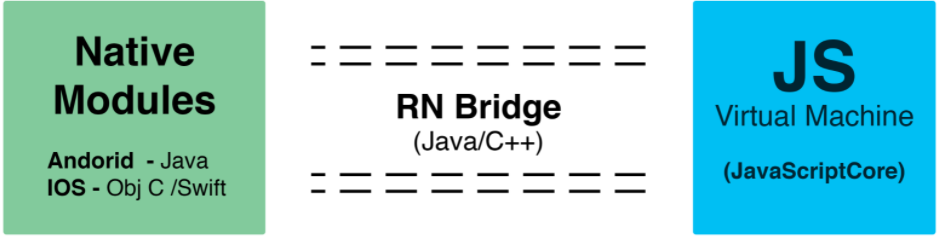
\includegraphics[width=1\textwidth]{figures/Aufbau_RN.png}
 \caption{Architektur React Native}
 \quelle{\cite{o.V..o.J.}}
 \label{fig:structure}
\end{figure}
%Zitat fehlt
Ersteres bietet in iOS JavaScriptCore und in Android eine Lösung, die von React Native zur Verfügung gestellt wird.
Dabei gibt es in React Native plattformübergreifende Abstraktionen wie \textit{View}, \textit{Image} oder \textit{NetInfo}, die korrespondierende Native Komponenten besitzen.
Die Bridge ist für die Kommunikation zwischen Native Module und JS-Umgebung verantwortlich.
Sie erhält von ersterem Events wie Toucheingaben oder Netzwerkanfragen und vom Native Module Anweisungen für das \ac{ui} oder \acp{api}.
Der Austausch findet dabei asynchron über \ac{json} statt.
Der letzte Teil der Architektur ist das Native Module.
Dies ist die Anwendung, die der Nutzer verwendet \cite{Behrends.2018}.
Es handelt sich somit bei Apps, welche mit React Native programmiert wurden, nicht um hybride Apps, da sie nicht nur in einem Native Container gerendert werden, sondern tatsächlich auf native Schnittstellen zugreifen.
Die Entwicklung solcher Apps ist dennoch plattformunabhängig, da die Implementierung in JavaScript erfolgt und die Umwandlung erst zur Laufzeit geschieht.
React Native Applikationen lassen sich dadurch schwierig in die bereits erklärten Kategorien von mobilen Anwendungen einordnen.%Siehe Seite 4 Behrends

Zur Nutzung von React Native Apps benötigt das Gerät mindestens iOS 11.0 oder Android 5.0 \cite{Facebook.d}.
Genau wie andere Native Apps können sie in den plattform-spezifischen App Store veröffentlicht und dort vom Nutzer heruntergeladen, installiert und aktualisiert werden.
Dabei ist der benötigte Signing-Prozess derselbe wie bei Native Applikationen.

Zur Implementierung von Komponenten und Funktionalitäten in React Native gibt es mehrere Optionen.
Die erste Option ist das Nutzen der bereits erwähnten \textit{Core Components}.
Weiterhin kann auf Community Lösungen zugegriffen werden, die Brücken zu nativen Schnittstellen implementieren.
Sollten die \textit{Core Components} nicht ausreichen, ist das meist die effizienteste Wahl, da viele Funktionalitäten bereits zufriedenstellend und stabil entwickelt und veröffentlicht wurden.
Unter \url{https://reactnative.directory/} sind diese Bibliotheken auffindbar und durch einen errechneten Directory Score nach mehreren Kriterien wie Beliebtheitskurve, Sterne auf GitHub oder Anzahl der Downloads bewertet.
Die letzte Option ist es, Native Modules selbstständig zu programmieren.
Das bedeutet, dass eine \textit{Bridge} zwischen React Native und der nativen Komponete implementiert werden soll, wodurch diese zur Laufzeit mit JavaScript angesprochen werden kann.
Somit ist es generell möglich alles was eine native Anwendung kann, auch in React Native umzusetzen.
 
% Erklärung RN: 2 threads: main thread und js thread. js theard sagt dem th über json, was es tun soll, mt hat ein riesen switch case, was die möglichen anfragen von jst beinhaltet und das dort dann den korrespondierenden java / objective-c code durchführt. theoretisch noch den diffing thread mit shadow dom, der dasselbe macht wie diffing in react. Hilft bei der Performance
\chapter{Kriterienkatalog zum Vergleich der Technologien}\label{ch:catalog}
Nach der Erläuterung der Grundlagen wird nun auf die Kriterien eingegangen, mithilfe denen die Technologien im Verlauf der Arbeit verglichen werden: Funktionalität, Kompatibilität mit verschiedenen Betriebssystemen und Entwicklungsaufwand der Anwendung.

Als Reaktion auf die Coronakrise soll eine App programmiert werden, die zur Darstellung und Durchsuchung der aktuellen COVID-19 Fallzahlen dient.
Dabei soll diese installierbar sein und auch bei schlechter oder fehlender Internetverbindung funktionieren.
Außerdem soll der Nutzer eine Filterung der Daten auf Basis seines aktuellen Standorts oder auf Basis der Adresse eines seiner Kontakte durchführen können.
Zuletzt soll es dem Nutzer möglich sein, Benachrichtigungen zur aktuellen Lage der Fallzahlen zu erhalten.

Anhand von Punkten wird die Erfüllung der Kriterien bemessen und zuletzt ausgewertet.
Dabei erfolgt bewusst ein Verzicht auf eine Gewichtung der Kriterien.
Der Grund hierfür ist, dass es sich in der vorliegenden Arbeit um einen Vergleich der Technologien handelt und deshalb alle Kriterien gleichbedeutend sind.

\section{Funktionalitäten}
Applikationen werden entwickelt, um Nutzern einen Mehrwert in ihrem Alltag zu bieten.
Je mehr Funktionalität eine Anwendung unterstützt, desto mehr Nutzen kann sie bieten.
Egal ob in der Web- oder Appentwicklung, wenn die Anwendung keinen Mehrwert bietet, wird sie nicht verwendet und wird dadurch vom Markt verdrängt.

Im Folgenden werden diejenigen Funktionalitäten von mobilen Anwendungen vorgestellt, die für den Vergleich ausgewählt wurden.

\subsection{Installation}
\subparagraph{Beschreibung\\}
Die Apps, die der Nutzer oft verwendet, sollten schnell erreichbar sein.
Eine Installation wird daher in vielen Fällen bevorzugt und stellt eine grundlegende Funktion von mobilen Anwendungen dar.\\
Dennoch bedeutet das Installieren für das verwendete Gerät, dass es Kapazität seines Speichers der Applikation zur Verfügung stellen muss.
Das ist dahingehend erwähnenswert, dass einige Nutzer auf das Installieren der App verzichten müssen, wenn ihnen unzureichend Speicherplatz zur Verfügung steht.

Falls nun Aktualisierungen des Herstellers verfügbar sind, möchte der Nutzer diese auch erhalten und durchführen können.
Dadurch können beispielsweise vorherige Fehler in der App bereinigt oder neue Funktionalität ermöglicht werden.

\subparagraph{Kriterium\\}
Mit diesem Kriterium soll geprüft werden, ob die Anwendung zur Nutzung installiert werden kann oder muss.

\begin{itemize}
\item 0 Punkte: Die Nutzung der Anwendung ist abhängig von deren Installation.
\item 1 Punkt: Die Nutzung der Anwendung ist unabhängig von deren Installation.
\end{itemize}

\subsection{Offlinebetrieb}
\subparagraph{Beschreibung\\}
Eine wichtige Funktion von mobilen Anwendungen ist der Offlinebetrieb.
Das bedeutet, dass die Anwendung auch ohne oder unter schlechter Internetverbindung verwenden werden kann.\\
Dabei muss unterschieden werden zwischen Anwendungen, die generell keinen Zugriff auf das Internet benötigen und jenen, die ihre Funktionalität im Offlinebetrieb einschränken.
Vorteil von letzterem ist auch, wenn die Prozesse, die im Offlinebetrieb angestoßen wurden, gehalten werden können, bis das Gerät wieder eine stabile Internetverbindung besitzt.
Auf diesem Wege wird gewährleistet, dass jegliche Aktivitäten erfolgreich durchgeführt werden.
Meistens bieten Applikationen eine Mischung aus beiden Optionen an.

Um aus technischer Sicht eine Unabhängigkeit von der Netzwerkverbindung zu schaffen, müssen Daten lokal in einem Speicher des Geräts abgelegt werden.
Das ermöglicht dem Nutzer, seine Daten jederzeit verfügbar zu haben und somit Abhängigkeiten von äußeren Umständen zu minimieren.

\subparagraph{Kriterium\\}
Dieses Kriterium soll prüfen, ob die Anwendung auch mit fehlender Netzwerkverbindung lauffähig ist.

\begin{itemize}
\item 0 Punkte: Die Anwendung ist nach der Installation ohne Netzwerkverbindung nicht lauffähig.
\item 1 Punkt: Die Anwendung ist nach der Installation ohne Netzwerkverbindung lauffähig.
\end{itemize}

\subsection{Standortzugriff}
\subparagraph{Beschreibung\\}
Um mobile Anwendungen auf die eigenen Bedürfnisse anzupassen, ist der Standortzugriff eine Option.
Dabei greift die Anwendung unter anderem durch das \ac{gps} auf den Standort des Nutzers zu und kann diesen weiterverarbeiten, um standortabhängige Informationen darzustellen.
Der Zugriff bezieht sie dabei auf den aktuellen Standort sowie auf Bewegungen des Nutzers.
Meist muss bereits während des Installationsprozesses der Applikation die Zustimmung des Nutzers für die Verwendung von standortbezogenen Inhalten eingeholt werden.
Wird dies genehmigt, ist es der Anwendung auch möglich, im Hintergrund auf \ac{gps}-Daten zuzugreifen.

Gängige Anwendungsfälle sind die Abfrage des Standorts für Wetterinformationen, Navigation oder die Anzeige von Dienstleistungen in der Nähe des aktuellen Standorts.

\subparagraph{Kriterium\\}
Dieses Kriterium betrachtet, ob die Anwendung Zugriff auf den Standort des Nutzers besitzt und diesen weiterverarbeiten kann.

\begin{itemize}
\item 0 Punkte: Die Anwendung besitzt keinen Zugriff auf den Standort des Nutzers.
\item 1 Punkt: Die Anwendung besitzt Zugriff auf den Standort des Nutzers.
\item 2 Punkte: Die Anwendung besitzt Zugriff auf den Standort des Nutzers und kann diesen selbstständig weiterverarbeiten, beispielsweise in Form von Geofencing\footnote{Geofencing bezeichnet das Auslösen von Benachrichtigungen beim Betreten oder Verlassen von definierten Bereichen und Orten.} oder Reverse Geocoding\footnote{Der Prozess, bei dem aus Informationen über Längen- und Breitengrad eine lesbare (Teil-)Adresse.}.
\end{itemize}

\subsection{Kontaktzugriff}
\subparagraph{Beschreibung\\}
Ein weiterer Zugriff auf native Schnittstellen eines mobilen Endgeräts bieten die Kontakte.
Diese sind meist auf dem Gerät oder dem verknüpften Google oder Apple Konto hinterlegt.
Sie können neben Bild, Name und Telefonnummer auch andere Kontaktdaten wie Anschriften oder E-Mail-Adressen beinhalten.

In vielen Nachrichtenübermittlungsspps wie WhatsApp, Telegram oder Kik Messenger werden diese Daten verarbeitet, um dem Nutzer die Möglichkeit zu geben, seine Kontakte abgesehen von SMS oder Anrufen zu kontaktieren.

\subparagraph{Kriterium\\}
Das Kriterium untersucht, ob die Anwendung Zugriff auf die Kontaktliste des Nutzers erhalten kann, um Kontaktdaten weiterzuverarbeiten.

\begin{itemize}
\item 0 Punkte: Die Anwendung besitzt keinen Zugriff auf die Kontakte des Endgeräts.
\item 1 Punkt: Die Anwendung besitzt Zugriff auf die Kontakte des Endgeräts.
\item 2 Punkte: Die Anwendung besitzt Zugriff auf die Kontakte des Endgeräts und kann Kontakte hinzufügen, verändern und löschen.
\end{itemize}

\subsection{Benachrichtigung}
\subparagraph{Beschreibung\\}
Benachrichtigungen sind heutzutage Bestandteil jeder App und spielen eine große Rolle bei der Interaktion mit den Nutzern.
Sie lassen sich aus technischer Sicht in zwei Kategorien unterteilen: nicht-persistente und persistent Benachrichtigungen.
Sie unterscheiden sich darin, dass erstere nur erscheinen, wenn die Anwendung in dem Moment in Benutzung ist, wohingegen das Empfangen von persistenten Benachrichtigungen jederzeit erfolgen kann.
Letztere können entweder von der Anwendung selbst oder von einem Server ausgelöst werden und werden deshalb auch als Push Benachrichtigungen bezeichnet.

Benachrichtigung können kurze Informationen durch Texte, Bilder oder Buttons beinhalten.
Letzteres ist besonders wichtig, da der Nutzer bei Push Benachrichtigungen über Buttons aus dem Menü heraus mit der Anwendung interagieren und auch auf diese weitergeleitet werden kann.\\
Außerdem könnten Benachrichtigungen Töne auslösen, um auf sich aufmerksam zu machen oder dem Icon der Anwendung ein Badge\footnote{Badges sind kleine Anzeigen am rechten oberen Rand des App Icons. An ihnen erkennt man die Anzahl an ungeöffneten Benachrichtigungen.} anheften.

Konkrete Beispiele für Inhalte von Benachrichtigungen sind aktuelle WhatsApp Nachrichten, neue Freundschaftsanfragen auf Facebook oder neue Suchergebnisse für die gespeicherte Ebay-Kleinanzeigen-Suche.

\subparagraph{Kriterium\\}
Die Anwendung muss fähig sein, Benachrichtigungen zu erhalten.
Dies sollte auch funktionieren, ohne dass die Anwendung im Vorder- oder Hintergrund geöffnet ist.

\begin{itemize}
\item 0 Punkte: Die Anwendung kann keine Benachrichtigungen erhalten.
\item 1 Punkt: Die Anwendung kann nicht-persistente Benachrichtigungen erhalten.
\item 2 Punkte: Die Anwendung kann persistente Benachrichtigungen erhalten.
\end{itemize}

\section{Kompatibilität mit verschiedenen Betriebssystemen}
\subparagraph{Beschreibung\\}
Durch die Vielzahl von Betriebssystemen und Geräten ist es aufwendig, Anwendungen zu implementieren, die überall im selben Maße lauffähig sind.
Projektleiter und Entwickler müssen deshalb im Voraus genau abwägen, auf welchen Systemen die Applikation verfügbar sein soll.\\
Hierbei kommt es bei Webanwendungen nicht nur auf das Betriebssystem, sondern auch auf den verwendeten Browser und dessen Version an.
Bei Android Geräten ist das vorinstallierte Browser Chrome und bei iOS Safari.
Auf welchen Geräten und Browsern die Anwendungen unterstützt werden sollen, wirkt sich außerdem direkt auf den Entwicklungsaufwand aus.

\subparagraph{Kriterium}
Das Kriterium besteht darin, dass die Anwendungen auf verschiedenen Betriebssystemen und Browsern funktionieren müssen.
Dabei ist ausschlaggebend, wie viele der bereits definierten Funktionalitäten auf dem Browser oder Betriebssystem verfügbar sind.

\begin{itemize}
\item 0 Punkte: Die Funktionalitäten der Anwendung sind mit einem Betriebssystem kompatibel und abhängig vom Browser.
\item 1 Punkt: Die Funktionalitäten der Anwendung sind mit einem Betriebssystem kompatibel und unabhängig vom Browser.
\item 2 Punkte: Die Funktionalitäten der Anwendung sind mit mehreren Betriebssystemen kompatibel und abhängig vom Browser.
\item 3 Punkte: Die Funktionalitäten der Anwendung sind mit mehreren Betriebssystemen kompatibel und unabhängig vom Browser.
\end{itemize}

\section{Entwicklungsaufwand}
\subparagraph{Beschreibung\\}
Bei der Implementierung von Anwendungen, egal ob für das Web oder für mobile Endgeräte, ist der Aufwand der Entwicklung ein maßgebender Faktor für resultierende Kosten.
Dabei fließen außerdem der Entwicklungszeitraum, die Fähigkeiten des Teams und der Funktionsumfang in die Kalkulation ein.
Wichtig ist, wie im vorherigen Kriterium angemerkt, auch die Kompatibilität mit verschiedenen Endgeräten.
Denn je mehr Geräte unterstützt werden sollen, desto aufwendiger und somit kostspieliger ist meist die Implementierung.

Wird jedoch zur Entwicklung ein plattformunabhängiger Ansatz gewählt, kann das bereits den Entwicklungsaufwand reduzieren.
Gerade wenn schnell reagiert werden soll -- zum Beispiel in der COVID-19-Krise -- ist es praktisch, wenn die Entwicklung möglichst effizient und die Anwendung auf vielen Geräten lauffähig ist, um ihre Nutzer effektiv zu unterstützen.

\acp{pwa} sind generell plattformübergreifend, da sie im Browser geöffnet werden.
Bei nativen Apps wird die Plattformunabhängigkeit durch Frameworks wie React Native ermöglicht.
Dennoch besteht bei beiden Ansätzen die Möglichkeit, dass zur Unterstützung von bestimmten, geforderten Betriebssystemen(-versionen) oder Browsern ein zusätzlicher Entwicklungsaufwand entsteht.

\subparagraph{Kriterium\\}
Auf Basis der bereits genannten Kriterien soll in diesem Kriterium gemessen werden, wie viel Zeit für deren Implementierung benötigt wird.
Dabei soll einerseits die Zeit zur Einarbeitung in die verschiedenen Technologien betrachtet werden sowie die tatsächliche Zeit, die zum Programmieren der Funktionalität benötigt wird.

\begin{itemize}
\item 0 Punkte: Der Einarbeitungs- und Programmieraufwand benötigt bei beiden Technologien gleich viel Zeit.
\item 1 Punkt: Der Einarbeitungs- oder Programmieraufwand benötigt weniger Zeit als bei der anderen Technologie.
\item 2 Punkte: Der Einarbeitungs- und Programmieraufwand benötigt weniger Zeit als bei der anderen Technologie.
\end{itemize}
\chapter{Implementierung einer Progressive Web App und Native App}\label{ch:implementation}
Die Daten für die zu implementierenden Applikationen werden von der offiziellen REST\footnote{Ein gängiges Datenformat des Datenaustauschs im Web.} \ac{api} des Robert Koch-Instituts bezogen.
Sie werden täglich um Mitternacht prozessiert und sind in den frühen Morgenstunden in der \ac{api} verfügbar.
Konkret wird die Datenbank \glqq RKI Corona Landkreise\grqq{} genutzt, die die Zahlen gruppiert nach Landkreisen im Geo\ac{json} und \ac{json}-Format zur Verfügung stellt.
Sie besitzt insgesamt 2.117.948 Datensätze und als CSV-Datei eine Größe von 308 MB\cite{COVID19Datenhub.2020}.\\
Für die Darstellung der Fallzahlen wurden hierbei folgende, auf den Landkreis bezogene, Attribute ausgewählt:
\begin{itemize}
\item Art des Landkreises (\textit{BEZ})
\item Name (\textit{GEN})
\item Fälle (\textit{cases})
\item Fälle der letzten 7 Tage pro 100.000 Einwohner (\textit{cases7\_per\_100k})
\item Fallzahlen pro 100.000 Einwohner (\textit{cases\_per\_100k})
\item ID (\textit{AdmUnitId})
\item Zeitpunkt der letzten Aktualisierung der Daten (\textit{last\_update})
\end{itemize}
In der Anwendung werden die Fallzahlen zum Zweck der Übersichtlichkeit auf zwei Nachkommastellen gerundet.

Für die Implementierung der zu vergleichenden Anwendungen wurden die open-source Bibliotheken React und React Native verwendet.
React dient bei der \ac{pwa} als Unterstützung zur Entwicklung einer \ac{spa}, wohingegen React Native ein komplettes Framework zur plattformunabhängigen Entwicklung von nativen Anwendungen anbietet.
Ein Vergleich mit diesen Bibliotheken bietet sich einerseits insofern an, dass deren Grundlage dieselbe Programmierweise darstellt, nämlich das deklarative und komponentenbasierte Konzept von React.
Anderseits sind durch die Verwendung von React Native beide Technologien plattformunabhängig und bilden somit eine solide Grundlage für den Vergleich.
Diese Eigenheit der Implementierung unterscheidet sich insofern grundlegend von der tatsächlichen nativen Entwicklung, als dass diese nicht betriebssystemspezifisch stattfindet.
Dafür muss die dafür vorgesehenen Programmiersprachen und ein \ac{ide} wie Android Studio mit Kotlin und Java genutzt werden.
Trotz dieser Besonderheit wird in der vorliegenden Arbeit eine React Native App als Native App mit einer \ac{pwa} verglichen, da sich generell mit React Native alle Funktionalitäten programmieren lassen, die Native Apps anbieten.

Das Besondere bei der Entwicklung einer Native App mit React Native ist, dass dies plattformunabhängig geschieht.
Wie bereits in Kapitel \ref{ch:basics} geschildert, handelt es sich dabei um einen Prozess, der von einem JavaScript Thread über \textit{Bridges} mit einem Native Thread kommuniziert und somit zur Laufzeit native Schnittstellen und \ac{ui}-Elemente aufruft.
Dadurch kann mit JavaScript Code geschrieben werden, der zur Laufzeit sowohl Android als auch iOS Komponenten anspricht.
Um eine Funktionalität mit JavaScript implementieren zu können, muss jedoch entweder bereits eine Community Lösung einer \textit{Bridge} für diese gewollte Funktion existieren oder diese selbst entwickelt werden.\\
Beide Applikationen sind im Quelltext-Editor Visual Studio Code und bis auf Ausnahmen bei der Native App mit JavaScript programmiert.

\section{Einrichten der Entwicklungsumgebung}
\subparagraph{Progressive Web App\\}
Zum Aufsetzen der Umgebung wurde die bereits genannte Create-React-App-Toolchain verwendet.
Diese wird durch npm\footnote{ehemals Node Package Manger, Anwendung zur Installation von Node.js Packages.} mit dem Befehl \textit{npx create-react-app <Name der Anwendung>} erstellt.
Hierfür wird mindestens Node\footnote{Node.js ist eine lizenzfreie und plattformunabhängige JavaScript Entwicklungsumgebung} 10.16 und npm 5.6 benötigt.
Nachteile der Verwendung einer Toolchain sind jedoch die Abhängigkeit von den dadurch integrierten Bibliotheken und das daraus resultierende Sicherheitsrisiko. 
Auf der anderen Seite ermöglicht die Toolchain einen schnellen Einstieg zur Entwicklung einer \ac{spa}.
Dies liegt vor allem an den vorgefertigten Konfigurationen zur Vereinfachung der Programmierung wie \textit{Babel}\footnote{Compiler, der mit ECMAScript 2015 geschriebenen Code rückwärtscompatibel macht durch dafür vorgesehene Polyfills.}, \textit{ESLint}\footnote{Codeanalysetool, welches den Entwickler auf problematische Codestellen aufmerksam macht.} und \textit{Webpack}\footnote{Modulbündler, der aus vielen einzelnen Dateien, ein oder mehrere große Dateien generiert. Dies erhöht die Performance der Anwendung.}.
Create-React-App bietet außerdem eine Reihe an Templates, die das Aufsetzen einer zum Projekt passenden Entwicklungsumgebung ebenfalls erleichtern sollen.
Beispielsweise das \ac{pwa} Template, das Werkzeuge wie \textit{Workbox}\footnote{Von Google entwickelte Sammlung von JavaScript Bibliotheken zur vereinfachten Implementierung von Service Workern.} und einen vorimplementierten Service Worker mitinstalliert.
Darauf wird in dieser Anwendung verzichtet, um die Funktionsweise des Service Workers selbst programmieren zu können und diese dadurch besser zu erfassen.

Die Abbildung \ref{fig:structure_pwa} zeigt die Ordnerstruktur nach dem Aufsetzen der Anwendung per Toolchain.
 
\begin{figure}[h]
 \centering
 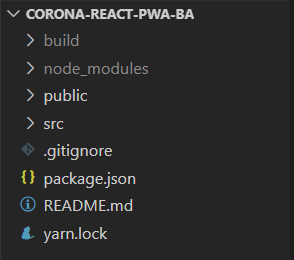
\includegraphics[width=0.6\textwidth]{figures/Structure_PWA.png}
 \caption{Ordnerstruktur Progressive Web App}
 \label{fig:structure_pwa}
\end{figure}

Im \textit{public}-Ordner befinden sich diejenigen Dateien, die an den Client versendet werden.
Konkret sind das ausgewählte Bilddateien, das App Manifest und die \textit{index.html}-Datei.
\textit{Webpack} nutzt die \textit{index.js} als Eintrittspunkt und generiert beim Ausführen der \textit{ReactDOM.render(element, document.getElementByID('root')}-Funktion einen Komponentenbaum auf dem \textit{div}-Element mit der \textit{id} \textit{root}.
Die \textit{index.js} befindet sich im \textit{src}-Ordner.
Auf ebendieser Ebene befindet sich außerdem die \textit{yarn.lock}, in der alle Abhängigkeiten der Anwendung gelistet sind, sowie die \textit{package.json}, die über Metadaten verfügt.

Mit dem Befehl \glqq npm run start\grqq{} wird eines der Skripte von Create-React-App zum Starten von \textit{Webpack} ausgeführt.
Dadurch ist die Anwendung direkt nach dem Aufsetzen unter \url{http://localhost:3000/} lokal aufrufbar.
Obwohl \text{localhost} kein \ac{https} besitzt, sind die Funktionalitäten von \acp{pwa} möglich, da es sich hierbei lediglich um die Entwicklungsumgebung handelt.

Zum Erhalten der Daten wird mit der \textit{Fetch}-Funktion eine \textit{GET}-Anfrage an die \ac{api} der Corona-Datenbank des Robert Koch-Instituts versendet und die Antwort in ein \textit{Array} gespeichert.
Dieses wird in der \textit{render}-Funktion mithilfe der \textit{Array}-Funktion \textit{map} durchlaufen.
Die Daten werden somit im \ac{ui} übersichtlich dargestellt.
%Bild der minimalen Ansicht

Generell müssen Webanwendungen auf einen Webserver veröffentlicht werden, um im World Wide Web aufrufbar zu sein.
Speziell bei \acp{pwa} ist hierbei bedeutsam, dass dieser Webserver eine verschlüsselte Verbindung mittels \ac{https} aufbaut, da dies eine technische Voraussetzung für \acp{pwa} ist.
Zum Hosting der Webapplikation wird deshalb der Hostingservice \textit{Netlify} verwendet, welcher eine \ac{https} Verbindung bereitstellt.
Durch den Befehl \glqq npm run build\grqq{} kann eine minimierte Version der Anwendung erzeugt werden, die eine optimierte Endfassung für das Deployment der App bietet.
Nach erfolgreichem Hochladen des Build Ergebnisses ist die \ac{pwa} über den Link \url{https://corona-react-pwa-ba.netlify.app/} verfügbar.

\subparagraph{React Native App\\}
Um eine React Native Anwendung zu programmieren, gibt es zwei Ansätze: \textit{managed workflow} und \textit{bare workflow}.
Ersteres wird durch das zusätzliche Expo Framework verwaltet, das einen schnellen Einstig in die plattformunabhängige Entwicklung ermöglicht.
Diese läuft mit der zugehörigen Expo Go iOS oder Android App, indem die programmierte App in Echtzeit über einen Packager gerendert wird.
Somit kann die App sofort ohne weiteres auf dem jeweiligen Endgerät unabhängig vom Betriebssystem getestet werden.\\
Der Nachteil dieses Ansatzes ist, dass mit Expo kein nativer Code für die genannten Betriebssysteme programmiert werden kann und dadurch die Funktionalitäten auf die von Expo angebotenen \ac{api}s beschränkt sind.
Für die Funktionen, die in dieser Arbeit betrachtet werden, würde Expo ausreichen, jedoch soll an dieser Stelle kein weiteres Framework genutzt werden.
Deshalb wird der \textit{bare workflow} verwendet.
%Auch hier kann mit JavaScipt (oder TypeScript falls gewünscht) programmiert werden, zusätzlich besteht aber auch die Möglichkeit nativen Code zu implementieren.
Doch auch dieser Ansatz besitzt einen Nachteil.
Denn trotz der eigentlich plattformunabhängigen Entwicklungsweise besteht keine Möglichkeit, mit Windows oder Linux eine iOS App zu programmieren.
Laut der Dokumentation von React Native wird hierfür macOS benötigt.\\
Im Folgenden wird daher die Implementierung einer Android App mit React Native beschrieben und die Umsetzung derselben Funktionalitäten auf iOS nur skizziert.
Wichtig ist dabei, dass aus dem vorliegenden Code trotzdem eine iOS App erzeugt werden könnte.
Die gleiche Funktionalität wie bei der Android App ist jedoch meist nicht ohne weitere Anpassungen wie das Zulassen von Berichtigungen über Apples \ac{ide} XCode verfügbar.

Zur Erstellung eines React Native Projekts wird der Befehl \textit{npx react-native init <Name der Anwendung>} verwendet, der ebenfalls von npm zur Verfügung gestellt wird.
Außerdem müssen diejenigen Einstellungen in der Entwicklungsumgebung vorgenommen werden, die auch zur Programmierung von nativen Android Apps benötigt werden.
Das betrifft beispielsweise das Installieren von Android Studio und der Android \ac{apk}.
Nach dem Ausführen des Befehls liegt die Ordnerstruktur vor, die in der Abbildung \ref{fig:structure_rn} dargestellt ist.

\begin{figure}[h]
 \centering
 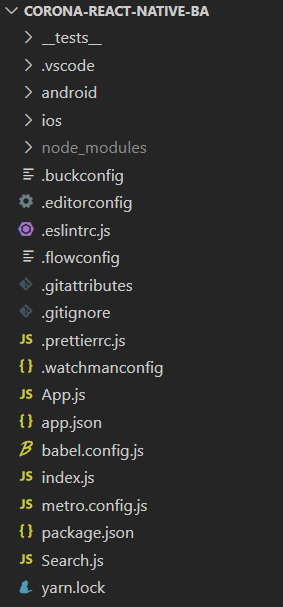
\includegraphics[width=0.4\textwidth]{figures/Structure_RN.png}
 \caption{Ordnerstruktur React Native App}
 \label{fig:structure_rn}
\end{figure}

Die Ordner \textit{ios} und \textit{android} beinhalten plattformspezifischen Code wie die \textit{Info.plist}- und die \textit{AndroidManifest.xml}-Datei, die Metainformationen über die Anwendung bereitstellen.
Auf derselben Ebene befindet sich die \textit{App.js}-Datei, in der die Anwendung mit JavaScript implementiert wird.

Um die Corona-Daten in der React Native App darzustellen, wird ebenfalls die \textit{Fetch} \ac{api} genutzt.
Diese verwendet die \textit{RCTNetworking}-Klasse als Bridge zu den nativen Modulen in Android und iOS.
In Android ist das der \textit{OkHttpClient} und in iOS \textit{XHTTP}.
Die Daten werden nach dem Abrufen durch die \textit{fetch}-Funktion in einer \textit{FlatList} angezeigt.
Der Vorteil der \textit{FlatList} ist, dass es nur diejenigen Elemente rendert, die im sichtbaren Teil des Bildschirms sind.
Dadurch werden Ressourcen gespart und das Scrollen der Liste erscheint für den Nutzer flüssiger.
Im Hintergrund spricht React Native mit der \textit{FlatList}-Komponente die Komponente \textit{ListView} in Android und in iOS an.
Die \textit{FlatList} wird umschlossen von einer \textit{SafeAreaView}-Komponente.
Dabei handelt es sich um eine iOS-spezifische Komponente, die empfohlen wird, um die \ac{ui} in iOS zu verbessern.
In der Abbildung \ref{fig:flatlist:ios} wird deutlich, welche Auswirkung das Fehlen dieser Komponente für die Benutzeroberfläche hat.

\begin{figure}
\subfigure[Darstellung einer \textit{FlatList} mit \textit{SafeViewArea}]{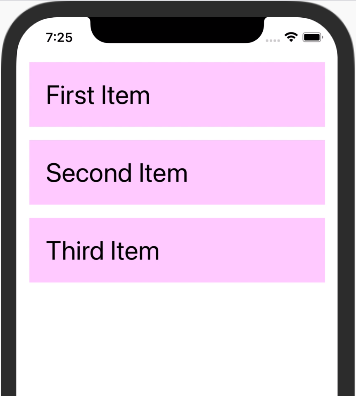
\includegraphics[width=0.49\textwidth]{figures/safeareaview.png}}
\subfigure[Darstellung einer \textit{FlatList} ohne \textit{SafeViewArea}]{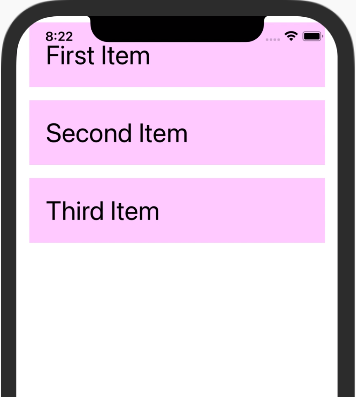
\includegraphics[width=0.49\textwidth]{figures/no_safeareaview.png}}
\caption{Exemplarische Darstellung einer Liste mit \textit{FlatList} in iOS}
\label{fig:flatlist:ios}
\end{figure}

Damit auf gewisse Funktionalitäten des Geräts zuzugreifen werden kann, benötigten Anwendungen teilweise die Erlaubnis des Nutzers.
Android unterscheidet dabei zwischen \glqq normal\grqq{} und \glqq dangerous\grqq{} \textit{Permissions}.
Beispiele für letzteres sind die \textit{android.permission.ACCESS\_""FINE\_LOCATION} oder \textit{android.permission.READ\_CONTACTS}.
Alle anderen \textit{Permissions} werden aus dem AndroidManifest.xml generiert.\\
Bei iOS Apps werden die benötigten Berechtigungen der App in XCode festgelegt und beim Installationsprozess abgefragt.
Nur wenn der Nutzer diese Berechtigungen akzeptiert, kann die Anwendung installiert werden.
Daher wird in der App für die Nutzung von Funktionalitäten wie Standort- oder Kontaktzugriff keine zusätzliche Erlaubnis des Nutzers benötigt.

\section{Installation und Aktualisierungen}

Das Ziel dieser Funktionalität ist es, dass die Anwendung auf das mobile Endgerät des Nutzers installiert werden kann.
Dadurch soll er schneller Zugriff ermöglicht werden.

\subparagraph{Progressive Web App\\}
Um eine Webanwendung installierbar zu machen, benötigt sie ein App Manifest und \textit{HTTPS}.
Für chromiumbasierte Browser ist außerdem ein Service Worker notwendig.
Dort bedeutet das Installieren in neueren Browserversionen, dass eine sogenannte WebAPK aus dem App Manifest generiert wird.
Somit ist diese dann auch unter allen Apps im App Drawer und den Einstellungen aufgelistet.
Dennoch ist sie Teil von Chrome und verliert beispielsweise ihre Daten, wenn die Cache-Daten von Chrome geleert werden.
Bei iOS Geräten bedeutet das Installieren lediglich ein Lesezeichen für die Anwendung zum Startbildschirm des mobilen Endgeräts hinzuzufügen, wie es auch mit herkömmlichen Webseiten und -anwendungen möglich ist.
Deshalb erscheint die App weder im App Drawer, noch unter den Einstellungen.

Wie bereits im Kapitel \ref{ch:basics} angemerkt, handelt es sich bei dem App Manifest um eine \ac{json}-Datei, die Informationen über die Anwendung bereitstellt.
Um das Installieren zu ermöglichen, muss dieses die in Abbildung \ref{lst:manifest} gezeigten Attribute beinhalten.
Ersteres gibt an, wie die Anwendung dargestellt werden soll.
Damit sie einer mobilen App gleicht, wird hier der Wert \textit{standalone} oder \textit{fullscreen} empfohlen.
Dadurch verschwindet die für Webanwendungen übliche \ac{url}-Leiste.
Durch die Angabe einer \textit{background\_color} erhält die Anwendung eine Hintergrundfarbe beim Starten der App.
Diese wird angezeigt, bis Stylingsheets oder Hintergrundbilder der PWA geladen sind.
Das \textit{icons}-Attribut besitzt ein Array aus Objekten, welche die Dateipfade der Icons in verschiedenen Größen angeben.
Die \textit{start\_url} gibt die relativen \ac{url} an, die beim Starten der installierten Anwendung geöffnet werden soll \cite{MDNcontributors.d}.\\
Das Manifest wird per \glqq <link>\grqq{}-Tag in die index.html eingebunden und dessen Informationen sind danach auch im Application-Tab der Google Developer Tools einsehbar \cite{Caceres.2021}.\\

\begin{lstlisting}[language=Java,caption={Fertiges App Manifest der PWA},captionpos=b,label={lst:manifest}]
{
  "name": "COVID-19 Fallzahlen",
  "icons": [
    {
      "src": "favicon.ico",
      "type": "image/x-icon",
      "sizes": "64x64",
    },
    {
      "src": "logo192.png",
      "type": "image/png",
      "sizes": "192x192"
    },
    {
      "src": "logo512.png",
      "type": "image/png",
      "sizes": "512x512"
    }
  ],
  "start_url": ".",
  "display": "standalone",
  "background_color": "#ffffff"
}
\end{lstlisting}

Wichtig ist dabei, dass das Manifest als experimentell markiert ist, da es nicht von allen mobilen Browsern und Betriebssystemen komplett unterstützt wird.
Aktuell betrifft das Safari, welches das Installieren aus Browsern, die auf iOS statt mit ihrem eigenen HTML-Renderer mit WebKit\footnote{HTML-Renderer von Safari.} laufen (Chrome, Firefox und Opera), nicht unterstützt \cite{o.V..}.
Denn jede iOS App muss laut Punkt 2.5.6 der Apple App Store Review Guidelines als Engine WebKit nutzen \cite{Apple.07.06.2021}.
Wenn der Nutzer nun die Anwendung im Browser aufruft, kann er sie auf browserabhängige Weise installieren und somit mit einem Klick vom Startbildschirm oder App-Drawer aus öffnen.
Beim Aufrufen der Seite, öffnet sich im Chrome Browser auf Android außerdem eine Installationsaufforderung für die App am unteren Bildschirmrand.
Diese zusätzliche Funktionalität muss aktuell für den Safari Browser explizit implementiert werden.

Für das Ermöglichen von Aktualisierungen der \ac{pwa} muss keine weitere Programmierung vorgenommen werden.
Sobald ein neues Deployment der Anwendung vorgenommen wird, ist sie automatisch auf dem neusten Stand, selbst wenn die \ac{pwa} installiert ist.

\subparagraph{React Native App\\}
Zur Ermöglichung der Installation einer React Native App bedarf es keiner konkreten Implementierung.
Es muss nur  -- wie bei nativen Anwendungen -- die betriebssystemabhängige Signierung durchgeführt werden.
Durch diesen Prozess erhält die Anwendung einen \textit{Release key} und einen \textit{Upload Key}, durch die sie eindeutig identifizierbar ist und auf die alle zukünftigen Aktualisierungen referenziert werden.
Die genauen Schritte sind in den offiziellen Dokumentationen von Apple und Android nachzulesen.
Zusätzliche Schritte für iOS, die eine Besonderheit von React Native sind, sind das Verbieten von HTTP Anfragen und das Umstellen der App im \textit{Release}-Schema.
Danach kann die resultierende \ac{apk}-Datei in den Google Play Store oder die \ac{ipa}-Datei in den Apple App Store hochgeladen werden.
Dort werden sie getestet und verifiziert.
Zuletzt kann der Nutzer sie im jeweiligen Store suchen und herunterladen.

Ähnlich wie bei der \ac{pwa} gibt es bei Android Apps die \textit{AndroidManifest.xml}-Datei, welche Informationen zur Installation der App bereitstellt, wie das App Icon, Berechtigungen der App oder die mindestens benötigte Android Version.
Bereits bei der Installation durch den Play Store wird dabei nach Berechtigungen für die Nutzung der App gefragt, die aus der AndroidManifest.xml ausgelesen werden.
Bei iOS Apps ist das die \textit{Info.plist}-Datei.

\section{Offlinebetrieb}

Die Anwendung soll auch ohne Internetverbindung aufrufbar, mit Daten gefüllt und die Funktion des Durchsuchens nutzbar sein.

\subparagraph{Progressive Web App\\}
Generell benötigten Nutzer eine Internetverbindung, um auf Webanwendungen zuzugreifen.
Durch moderne Webschnittstellen ist mittlerweile auch den Offlinebetrieb ermöglichen.
Hierfür wird der Service Worker genutzt.
Er kann auf eine statische, individuelle Seite weiterleiten, welche die standardmäßig angezeigte Seite bei fehlender Internetverbindung ersetzt.
Alternativ können aber durch den Service Worker auch Daten abgespeichert und im Offlinebetrieb angezeigt werden.
Hierfür gibt es neben der bereits seit 2015 bestehenden \textit{IndexedDB} auch die Cache \ac{api}, mit der Daten als Request-Response-Paar abgespeichert werden können.
Aus einer Vielzahl von clientseitigen Speichermechanismen im Web (\textit{LocalStorage}, \textit{SessionStorage} oder \textit{Cookies}) eignen sich speziell diese beiden zur Nutzung in einer \ac{pwa}.
Das ist damit zu begründen, dass sie persistent sein können und asynchron ablaufen \cite{LePage.2020}.
Letzteres verhindert, dass der Main Thread der Webanwendung blockiert wird und die Nutzer unter Umständen lange Warte- /Ladezeiten bei der Bedienung der Anwendung erfahren.
Gerade die Cache \ac{api} wird jedoch im Zusammenhang mit \acp{pwa} besonders empfohlen, weil diese im Gegensatz zur \textit{IndexedDB} auch statische Ressourcen speichert \cite{MDNcontributors.o.J.}.
Die Speichergröße von beiden Speichern ist abhängig von dem Browser, in dem die Webanwendung aufgerufen wird.

Durch das Zwischenspeichern der Daten wird ermöglicht, dass die \ac{pwa} dem Nutzer selbst ohne oder mit schlechter Internetverbindung Rückmeldung in Form einer Benutzeroberfläche zur Verfügung stellt.
Das kann entweder eine individuelle Seite oder dieselbe Seite mit veralteten Daten sein.
Ferner ist das Caching der Daten zum Offlinebetrieb der Anwendung nicht nur hilfreich, wenn keine Internetverbindung besteht, sondern reduziert auch allgemein die Anfragen an den Server. %Quelle

Eine Anwendung kann mehrere Caches besitzen, die zur Unterscheidung benannt werden.
In der programmierten \ac{pwa} werden an zwei Stellen Daten im \textit{cache-v1}-Cache gespeichert.
Zuerst geschieht dies beim Installieren des Service Workers im \textit{install}-Lifecycle-Event.
Hier werden statische Ressourcen wie das Manifest und Bilddateien in den Cache aufgenommen.\\
Die zweite Stelle ist während des \textit{fetch}-Events zur Speicherung von Netzwerkabfragen.
Dabei ist nicht nur die Speicherung von Bedeutung, sondern auch wie dieses Cache-Daten in der \ac{pwa} genutzt werden.
Hierfür definiert Jake Archibald mehrere Strategien, wovon die \glqq Cache, falling back to network\grqq{}-, \glqq Network, falling back to cache\grqq{}- und \glqq Cache then network\grqq{}-Strategie ausgewählt und für diesen Anwendungsfall untersucht wurden \cite{Archibald.2020}.

\begin{figure}
\centering
    \subfigure[Cache, falling back to network]{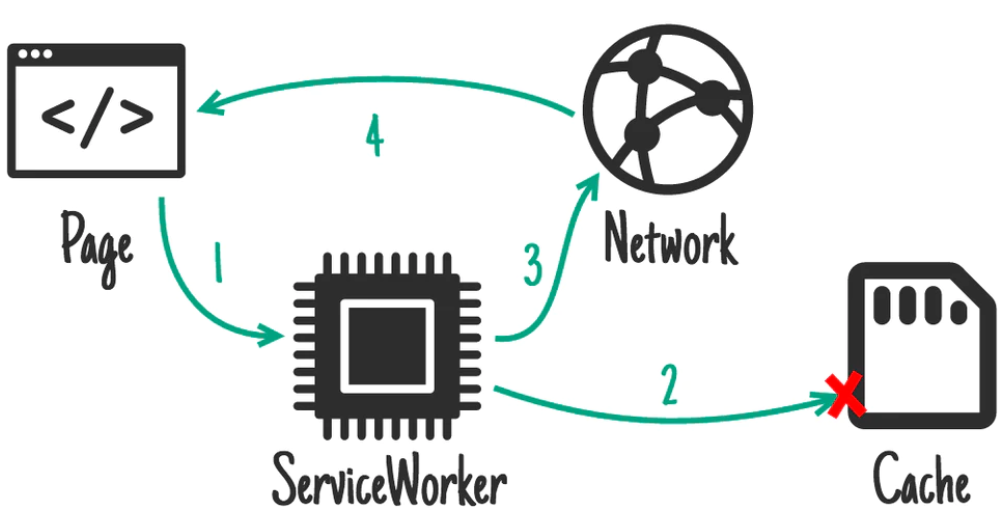
\includegraphics[width=0.49\textwidth]{figures/Cache_falling_back_to_network.png}}
        \subfigure[Network, falling back to cache]{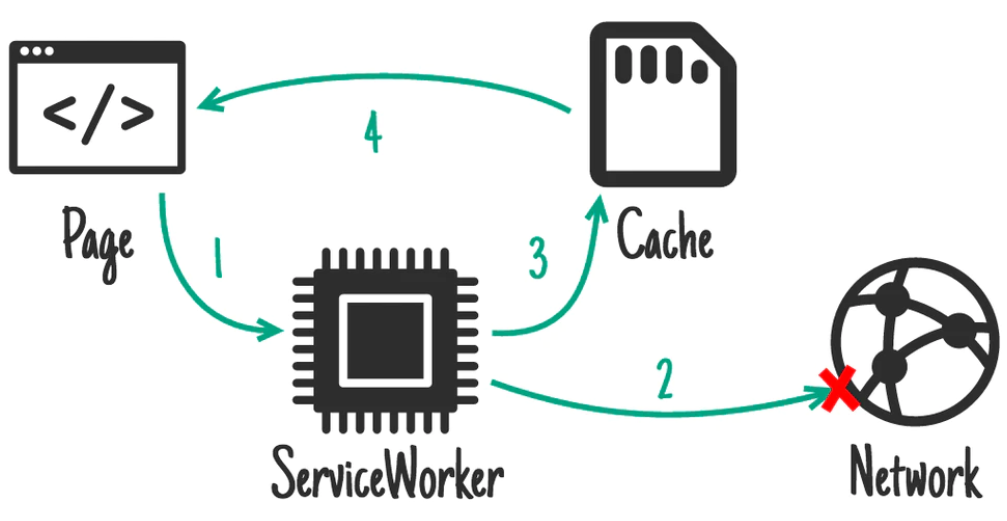
\includegraphics[width=0.49\textwidth]{figures/Network_falling_back_to_cache.png}}
    \subfigure[Cache then network]{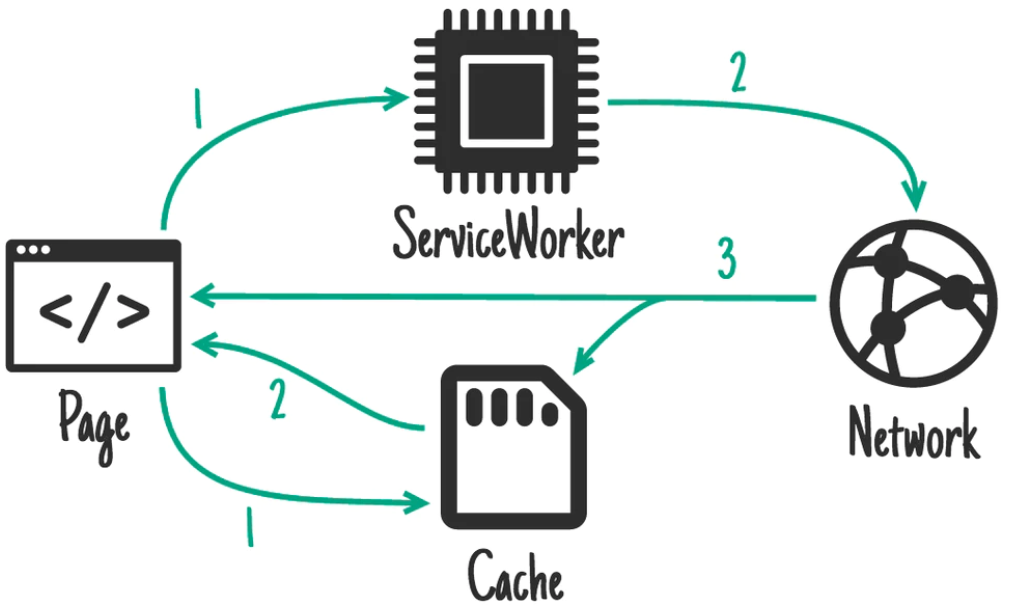
\includegraphics[width=0.49\textwidth]{figures/Cache_then_network.png}}
\quelle{\cite{Archibald.2020}}
\caption{Speichermanagementstrategien}
\end{figure}

Ersteres bedeutet, dass der Service Worker beim Ausführen der Anwendungen zuerst prüft, ob die Daten im Cache-Speicher verfügbar sind, und wenn dies nicht zutrifft, eine Netzwerkanfrage stellt.
Die Anwendung ist dadurch performant, der Nachteil ist jedoch, dass die Daten beim Aufrufen der App nicht auf dem aktuellsten Stand sind.\\
Zweiteres verfolgt einen gegenteiligen Ansatz, bei dem nur im Falle einer fehlenden Netzwerkverbindung die Daten aus dem Cache verwendet werden.
Auf diese Weise sind die Daten stets aktuell, jedoch erhöht sich auch die Anzahl an Netzwerkanfragen und somit der Verbrauch von Datenvolumen, gerade bei dieser großen Datenmenge, die vom Robert Koch-Institut zur Verfügung gestellt wird.
Außerdem muss der Nutzer warten, bis die Netzwerkanfrage fehlschlägt, bis die Cache-Daten genutzt werden.
Dies kann für Nutzer mit geringer Internetverbindung länger dauern und dadurch die Nutzererfahrung verschlechtern.\\
Der \glqq Cache then network\grqq{}-Ansatz stellt gleichzeitig eine Anfrage an den Cache und eine an das Netzwerk.
Sobald die Daten aus dem Cache geladen sind, werden sie in der Anwendung dargestellt.
In jedem Fall werden die Daten aber auch nach Antwort der Netzwerkanfrage im Cache aktualisiert \cite{Archibald.2020}.
Diese Variante benötigt eine Implementierung im Service Worker und in der Anwendung selbst, um zwei Anfragen auszulösen.

Die Entscheidung fiel zuletzt auf den \glqq Cache then network\grqq{}-Ansatz, mit einer zusätzlichen Besonderheit.
Denn dadurch, dass bei der Anwendung einerseits die Aktualität der Daten eine große Rolle spielt, anderseits die Daten sich nicht über den Tag hinweg ändern, ist eine ständige zweite Anfrage an das Netzwerk redundant.
Deshalb ist in der Anwendung eine Abfrage implementiert, welche prüft, ob das Datum der Robert Koch-Institut-Daten mit dem heutigen übereinstimmt.
Nur wenn dies nicht zutrifft, wird eine Anfrage an das Netzwerk gestellt und daraufhin die Daten im Cache aktualisiert.

Durch das Zwischenspeichern der Daten wird ermöglicht, dass die \ac{pwa} dem Nutzer selbst ohne oder mit schlechter Internetverbindung Rückmeldung in Form einer Benutzeroberfläche zur Verfügung stellt.
Das kann entweder eine individuelle Seite oder dieselbe Seite mit veralteten Daten sein.
In der implementierten \ac{pwa} ist letzteres der Fall und über eine Zeitstempel erfährt der Nutzer die Aktualität der angezeigten Daten.
Hierbei ist wichtig anzumerken, dass der Offlinebetrieb nur dann gewährleistet ist, wenn der Service Worker bereits auf dem Gerät installiert ist.
Dies ist der Fall, wenn die Anwendung in einem Browser-Tab geöffnet ist oder auf den Startbildschirm heruntergeladen wurde.

\subparagraph{React Native App\\}
Mobile Anwendungen sind im Gegensatz zu \acp{pwa} generell offline aufrufbar.
Der Grund dafür ist, dass das Rendern der App nicht abhängig von einer Netzwerkverbindung ist, weil sie bereits auf dem Endgerät existiert.
Dennoch ist es sinnvoll, auch hier eine lokale Speicherung der Corona-Daten vorzunehmen, um diese trotz Offlinebetriebs anzeigen zu können.

Seit React Native Version 0.59 sind einige Komponenten als veraltet deklariert.
Das betrifft unter anderem \textit{AsyncStorage} und \textit{NetInfo}.
Sie wurden jedoch nicht entfernt, sondern lediglich aus der Kernbibliothek react-native exkludiert und in jeweils eigene Bibliotheken mit eigenen Verantwortlichen verschoben \cite{Turner.2019}.
Diese Bibliotheken sind dem GitHub Repository @react-native-community zu finden und benötigen nach der Installation per npm auch das React Native-spezifische \textit{Linkings}\footnote{Ein Prozess bei dem diejenigen nativen Fähigkeiten, die von einer Bibliothek benötigt werden, der Anwendung hinzugefügt werden. Durch diesen zusätzlichen Schritt verringert sich die Größe der Basis Anwendungen, die eventuell keine nativen Funktionalitäten benötigt.}.

Der \textit{AsyncStorage} legt persistent Daten unverschlüsselt in einem lokalen Speicher ab.
Der Speicherplatz ist dabei standardmäßig auf 6 MB beschränkt, allerdings kann dieser auch manuell erweitert werden \cite{Behrends.2018}.
Die Daten werden bei iOS Geräten im \textit{Application Support}-Verzeichnis abgelegt.
In Android wird für die asynchrone Speicherung \textit{SQLite} verwendet.

Die Implementierung der Speicherung erfolgt nach der \glqq Network, falling back to cache\grqq{}-Strategie.
Demnach wird erst abgefragt, ob das Gerät eine aktive Internetverbindung besitzt und wenn dies fehlschlägt, die Daten aus dem \textit{AsyncStorage} verwendet.\\
Dafür stellt die \textit{NetInfo}-Komponente Informationen zur aktuellen Netzwerkverbindung bereit.
Diese wird genutzt um im Falle einer fehlenden Internetverbindung, die Corona-Daten aus dem \textit{AsyncStorage} zu entnehmen.\\
Zuerst werden jedoch die Daten nach erfolgreicher \ac{api}-Abfrage im \textit{AsyncStorage} gespeichert.
Eine Anforderung dabei ist, dass sie vorher in ein \ac{json}-String konvertiert werden müssen.

Im initialen \textit{useEffect}-Hook wird beim nächsten Aufruf der App geprüft, ob eine Internetverbindung besteht.
Wenn dies nicht zutrifft, wird per asynchroner Funktion auf die Daten im \textit{AsyncStorage} zugegriffen.
Sobald die Internetverbindung wiederhergestellt ist, werden die Daten per Netzwerkanfrage von der \ac{api} abgerufen.
%Außerdem wird ein weiterer \textit{useEffect} hinzugefügt, der auf Änderungen der \textit{NetInfo} hört und dementsprechend die Daten neu lädt.
%Somit wird gewährleistet, dass der Nutzer die neusten verfügbaren Corona-Daten erhält, wenn er eine Netzwerkverbindung hat.

Zum Testen des Offlinebetriebs muss nun das Internet des Rechners, auf dem der Emulator geöffnet ist, ausgeschaltet werden.
Dadurch wird nachgewiesen, dass die Anwendung trotz fehlender Netzwerkverbindung, die im \textit{AsyncStorage}-gespeicherten Corona-Daten anzeigen kann.

\section{Standortzugriff}

Anhand des Standorts soll der Nutzer die Liste der Landkreise nach dem Landkreis filtern, in dem er sich aktuell befindet.

\subparagraph{Progressive Web App\\}
Der Standortzugriff wird im Web über die sogenannte Geolocation \ac{api} ermöglicht.
Die Bestimmung erfolgt dabei unter anderem durch GPS und verschiedenste Netzwerksignale.
Sie wird vom \textit{navigator}-Objekt zur Verfügung gestellt und bietet unter anderem Zugriff auf Längen- und Breitengrad, Genauigkeit des bestimmten Standorts und die Höhe über dem Meeresspiegel des Gerätes \cite{Caceres.2021b}.

Zur Implementierung dieser Funktionalität wird der Nutzer beim Klicken des \glqq Standort bestimmen\grqq{}- Buttons zuerst, wie in Abbildung \ref{fig:permission_safari} zu sehen, nach seiner Zustimmung gefragt.

\begin{figure}[h]
 \centering
 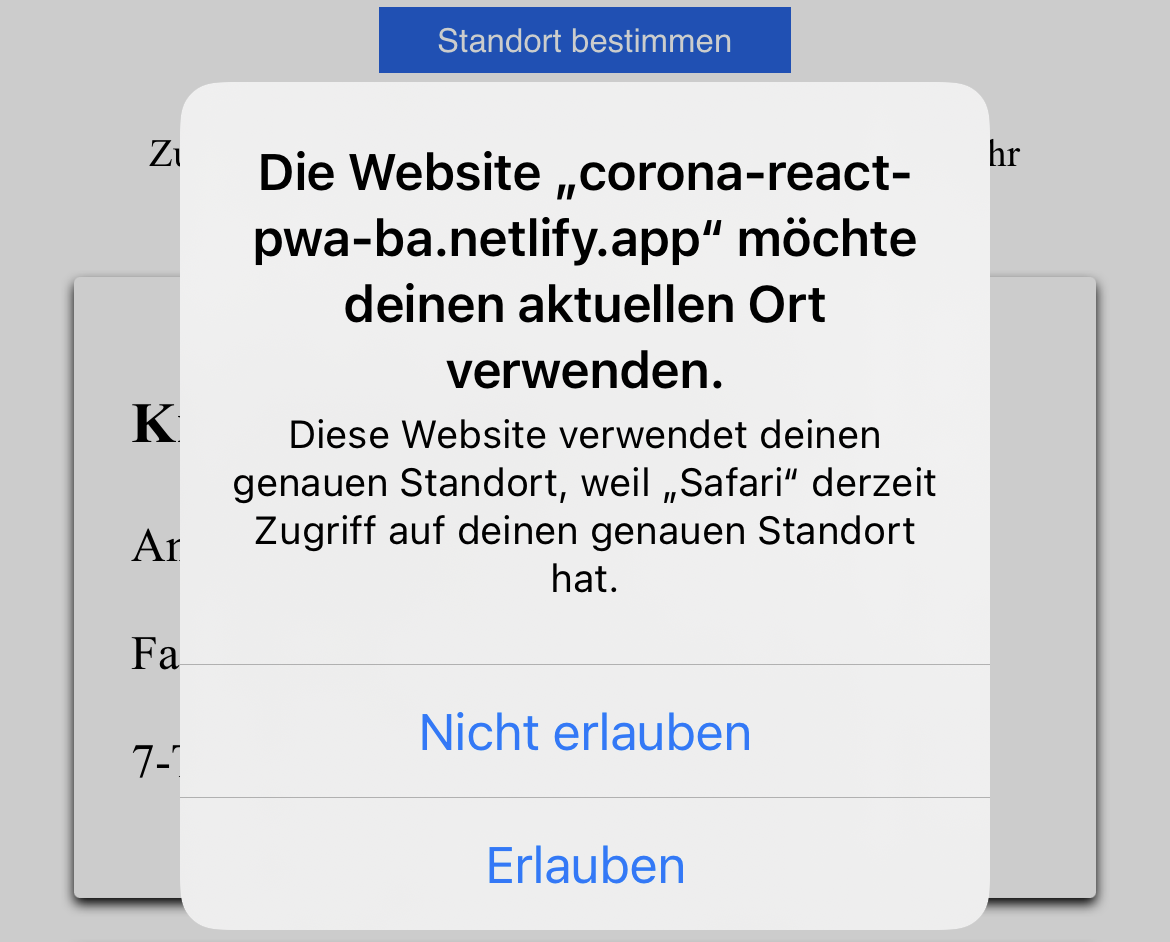
\includegraphics[width=0.6\textwidth]{figures/Permission_Safari.png}
 \caption{Erfragung des Standortzugriffs im iOS Browser}
 \label{fig:permission_safari}
\end{figure}

Sobald diese erteilt ist, wird die Methode \textit{Navigator.getCurrentPosition()} aufgerufen und deren Rückgabewert -- ein Objekt des Typs \textit{GeolocationPosition} -- einer Variablen zugewiesen.\\
Über eine kostenfreie Drittanbieter \ac{api} wird durch den Prozess des Reverse Geocachings aus den \textit{location.coords.latitude} und \textit{location.coords.longitude} Daten die Aufenthaltsstadt bestimmt.
Der Wert des \textit{input}-Feldes wird dann auf den ermittelten Landkreis gesetzt und die Liste der Landkreise automatisch nach dieser gefiltert.

\subparagraph{React Native App\\}
Zur Implementierung des Standortzugriffs in React Native wird die Community Lösung \textit{react-native-geolocation-service} verwendet, welche nach Aussage des Erstellers für Android und iOS programmiert ist.
Diese greift über eine \textit{Bridge} auf diejenigen Schnittstellen zu, die in Android und in iOS verantwortlich für den Standort sind.
In Android wird speziell wegen eines Timeout-Problems nicht auf die übliche \textit{Geocoder}-Klasse zugegriffen, sondern auf die \textit{FusedLocationProviderClient} \ac{api} des Google Play Services. %Quelle
%Die korrespondieren Klasse, die in iOS der Standortzugriff ermöglicht, nennt sich \textit{RCTGeolocation}.
%Über eine \textit{Bridge} wird die Kommunikation zwischen \textit{Main Thread} und \textit{JS Thread} gehandhabt.
In iOS spricht die \textit{Bridge} den \textit{CLLocationMangager} des \textit{CoreLocation}-Modules an.

Nach dem Installieren der Bibliothek muss für Android das Codefragment \textit{<uses-permission android:name="android.permission.ACCESS\_FINE\_LOCATION"/>} in der AndroidManifest.xml hinzugefügt werden.
Das erlaubt der Anwendung auf den Standort zuzugreifen, wenn die App benutzt wird.
%für iOS zusätzlich der Wert \textit{NSLocationWhenInUseUsageDescription} in der Info.plist-Datei gesetzt werden.
Da es sich beim Standortzugriff um eine \glqq dangerous\grqq{} \textit{Permission} handelt, muss zuerst der Nutzer dennoch erst eine Erlaubnis erteilen. 
Dies geschieht mit dem Befehl \textit{PermissionAndroid.request()}.
Für iOS wird neben dem Aktivieren des Standortzugriffs in XCode keine explizite Erlaubnis benötigt.

Die Abfrage der Erlaubnis erfolgt in der \textit{Search.js} in einem \textit{Effect}, welcher beim Öffnen der Anwendung ausgelöst wird.
Nach Zustimmung des Anwenders wird per \ac{api}-Anfrage an denselben Drittanbieter wie bei der \ac{pwa} der Name der Stadt aus den Daten über den Längen- und Breitengrad des Standorts des aktuellen Geräts erschlossen.
Hierbei ist zu betonen, dass im Normalfall bei nativen Anwendungen nach der Standortbestimmung auf die betriebssystemintegrierte Reverse Geocoding Funktion (beispielsweise bei Android die Google Maps Geocoding \ac{api}) zurückgegriffen werden könnte.
In dieser Arbeit wird jedoch wegen der dadurch anfallenden Kosten darauf verzichtet.

Der logische Aufbau dieser Funktionalität konnte hier von der React \ac{pwa} übernommen werden, lediglich die Events wurden abgeändert.
So nennt sich das \textit{onChange}-Event einer Texteingabe in React nun \textit{onChangeText}-Event in React Native, während das \textit{input}-HTML-Element zum \textit{TextInput}-Tag wird.

\section{Kontaktzugriff}

Dem Nutzer soll es möglich sein, die Liste der Landkreise nach der Adresse eines Kontakts zu filtern.

\subparagraph{Progressive Web App\\}
Die Kontakte eines mobilen Endgeräts stehen der Webanwendung über das \textit{navigator}-Interface zur Verfügung.
Konkret ist es dessen \textit{contacts}-Property, dass in chromiumbasierten Browsern seit Version 80 die Contact Picker \ac{api} implementiert und im \ac{https} Kontext nutzbar ist.
Falls kein \ac{https} vorhanden ist, existiert das Property nicht im \textit{navigator}.

Mittels der \textit{select}-Funktion kann ein Kontakt auf Basis des Namens ausgewählt werden.
Dabei wird bei der Implementierung festgelegt, welche Kontaktdaten bei der Auswahl angezeigt werden.
In der \ac{pwa} soll nun aus der Adresse des Kontakts die Stadt entnommen und dieser Wert in das Suchfeld gesetzt werden.
Dadurch wird die Liste der Landkreise nach der Stadt der Adresse des Kontakts gefiltert.
Die \textit{address} eines Kontakts besitzt die gleichen Werte wie die des \textit{PaymentAddress}-Interfaces, das aus der Payment Request \ac{api} bekannt ist.
Diese sind beispielsweise \textit{city}, \textit{country} und \textit{region}.

Auch für diesen Eingriff in die Kontaktliste des Nutzers muss explizit eine Erlaubnis erteilt werden.
Die Abfrage erfolgt beim Betätigen des Buttons und ist wie beim Standortzugriff eine browserbasierte Abfrage.

Das Implementieren dieser Funktionalität gestaltet sich als problematisch, da die Contact Picker \ac{api} lediglich auf mobilen Browsern zur Verfügung steht.
Deshalb wurde die Funktion vollständig mit dem Android Emulator programmiert.
Dafür wird statt durch \textit{http://localhost:3000} mit der IP-Adresse auf die laufende Webanwendung zugegriffen.
Doch auch hier gibt es Komplikationen mit der Unterstützung des \textit{contacts}-Attribut im \textit{navigator}.
Zuletzt hat lediglich das Deployment der \ac{pwa} geholfen, auf die Kontakte zuzugreifen.
Grund dafür kann sein, dass die Contact Picker \ac{api} nur mit \ac{https} verfügbar ist, jedoch sollte das nicht für \textit{localhost} gelten, wie bei der Implementierung der bisherigen Funktionalitäten.
Durch die Bestätigung der Sucheingabe wird in einer Funktion der Code in Abbildung \ref{lst:contacts} ausgeführt.

\begin{lstlisting}[language=Java,caption={Zugriff auf Kontakte},captionpos=b,label={lst:contacts}]
const props = ["name", "address"];
if ("contacts" in navigator) {
	try {
		const contact = await navigator.contacts.select(props, {});
        onQueryChange(contact[0].address[0].addressLine[0]);
		// Further processing
	} catch (ex) {
		// Handle any errors here.
	}
} else {
	// Handle no support
}
\end{lstlisting}

Mit dem Befehl \textit{navigator.contacts.select(props,{})} kann auf die Kontaktliste eines Geräts zugegriffen werden.
Der erste Übergabeparameter ist dabei ein \textit{Array} mit denjenigen Attributen, welche angezeigt werden sollen, während der Zweite weitere Konfigurationen wie beispielsweise eine Mehrfachauswahl von Kontakten zulässt.
Der Rückgabewert ist in diesem Falle ein \textit{Array}, dass einen Kontakt enthält.
Per \textit{address[0]} wird auf die erste Adresse des Kontakts zugegriffen.
Eigentlich kann daraufhin durch \textit{.city} die Stadt dieser Adresse erreicht werden, jedoch erlaubt der verwendete Emulator bei der Erstellung eines Kontakts nur die Eingabe der Adresse in eine Eingabezeile.
Deshalb wird hier auf die Adresszeile zugegriffen, in der zur Vereinfachung aktuell nur die Stadt notiert ist.
Dieser Wert wird nach Bestätigung der Auswahl direkt in das Suchfeld übernommen und die Liste der Landkreise somit nach dieser Stadt gefiltert.

\subparagraph{React Native App\\}
Bei der React Native App wurde dies mit der Bibliothek \glqq react-native-contacts\grqq{} umgesetzt.
Diese greift in Android auf die \textit{ContactsContract} Klasse und in iOS auf die \textit{CNContact} zu.

Nach der Installation der Bibliothek müssen in der AndroidManifest-Datei erneut eine \textit{uses-permissions} ergänzt werden, in diesem Fall die \textit{android.permission.READ\_""CONTACTS}-Erlaubnis für das Lesen der Kontakte.
Da es sich auch hierbei um ein \glqq dangerous\grqq{} Berechtigung handelt, muss erneut zuerst nach der Erlaubnis des Nutzers gefragt werden.
Dies wird in einer \textit{asnyc}-Funktion erledigt.
Sie wird in einem \textit{Modal} aufgerufen, in dem nach dem Namen des gesuchten Kontakts gefragt wird.
Nach der Betätigung des \textit{Bestätigen}-Buttons wird nun mit der Funktion \textit{Contact.getContactsMatchingString(text)}, die als Übergabeparameter einen \textit{string} annimmt, ein Kontakt gesucht, der diesen Übergabeparameter als Teil seines Namens enthält.\\
Das Ergebnis ist ein \textit{Array} aus Objekten von Kontakten, auf die das Kriterium zutrifft.
Zur Vereinfachung der Implementierung wird nur der erste Kontakt betrachtet und aus dessen \textit{postalAddresses} die erste Adresse ausgewählt.
Diese wird dann per Aufruf von \textit{onQueryChange} automatisch in das Suchfeld gesetzt und somit die Liste der Landkreise nach dieser Stadt gefiltert.\\
Bei der Implementierung wurde einige Mal keine Daten angezeigt und die Console beinhaltete \glqq {"\_U": 0, "\_V": 0, "\_W": null, "\_X": null}\grqq{}.
Es stellte sich heraus, dass dies damit verbunden ist, dass beim Anfordern der Ressourcen nicht auf das Auflösen des \textit{Promises} gewartet wurde.
Das konnte mit dem Schlüsselwörtern \textit{await} in den asynchronen Funktionen gelöst werden.

\section{Benachrichtigungen}
Die entwickelte App soll seinen Abonnenten Benachrichtigungen senden können.
In diesen können beispielsweise aktuelle Veränderungen der Inzidenz oder Informationen über neue Fallzahlen angezeigt werden.

Wie in Kapitel \ref{ch:basics} beschrieben, lassen sich Benachrichtigungen in nicht-persistente und persistente Benachrichtigungen unterteilen.
Im Zuge dieser Arbeit soll nun erklärt werden, wie letzteres umgesetzt werden kann, da diese eine höhere Relevanz zur Interaktion mit dem Nutzern bieten und hierfür auch Schnittstellen genutzt werden, die von nicht-persistente Benachrichtigungen verwendet werden.
Somit wird auf die Nutzung beider Arten eingegangen.

Für beide Anwendungen muss ferner das Management der Nutzererlaubnis implementiert werden.
Dies wird zur Begrenzung des Umfangs in der Arbeit exkludiert und im Folgenden lediglich auf die Programmierung der Push Benachrichtigungsfunktion selbst eingegangen.

\subparagraph{Progressive Web App\\}
\begin{figure}[h]
 \centering
 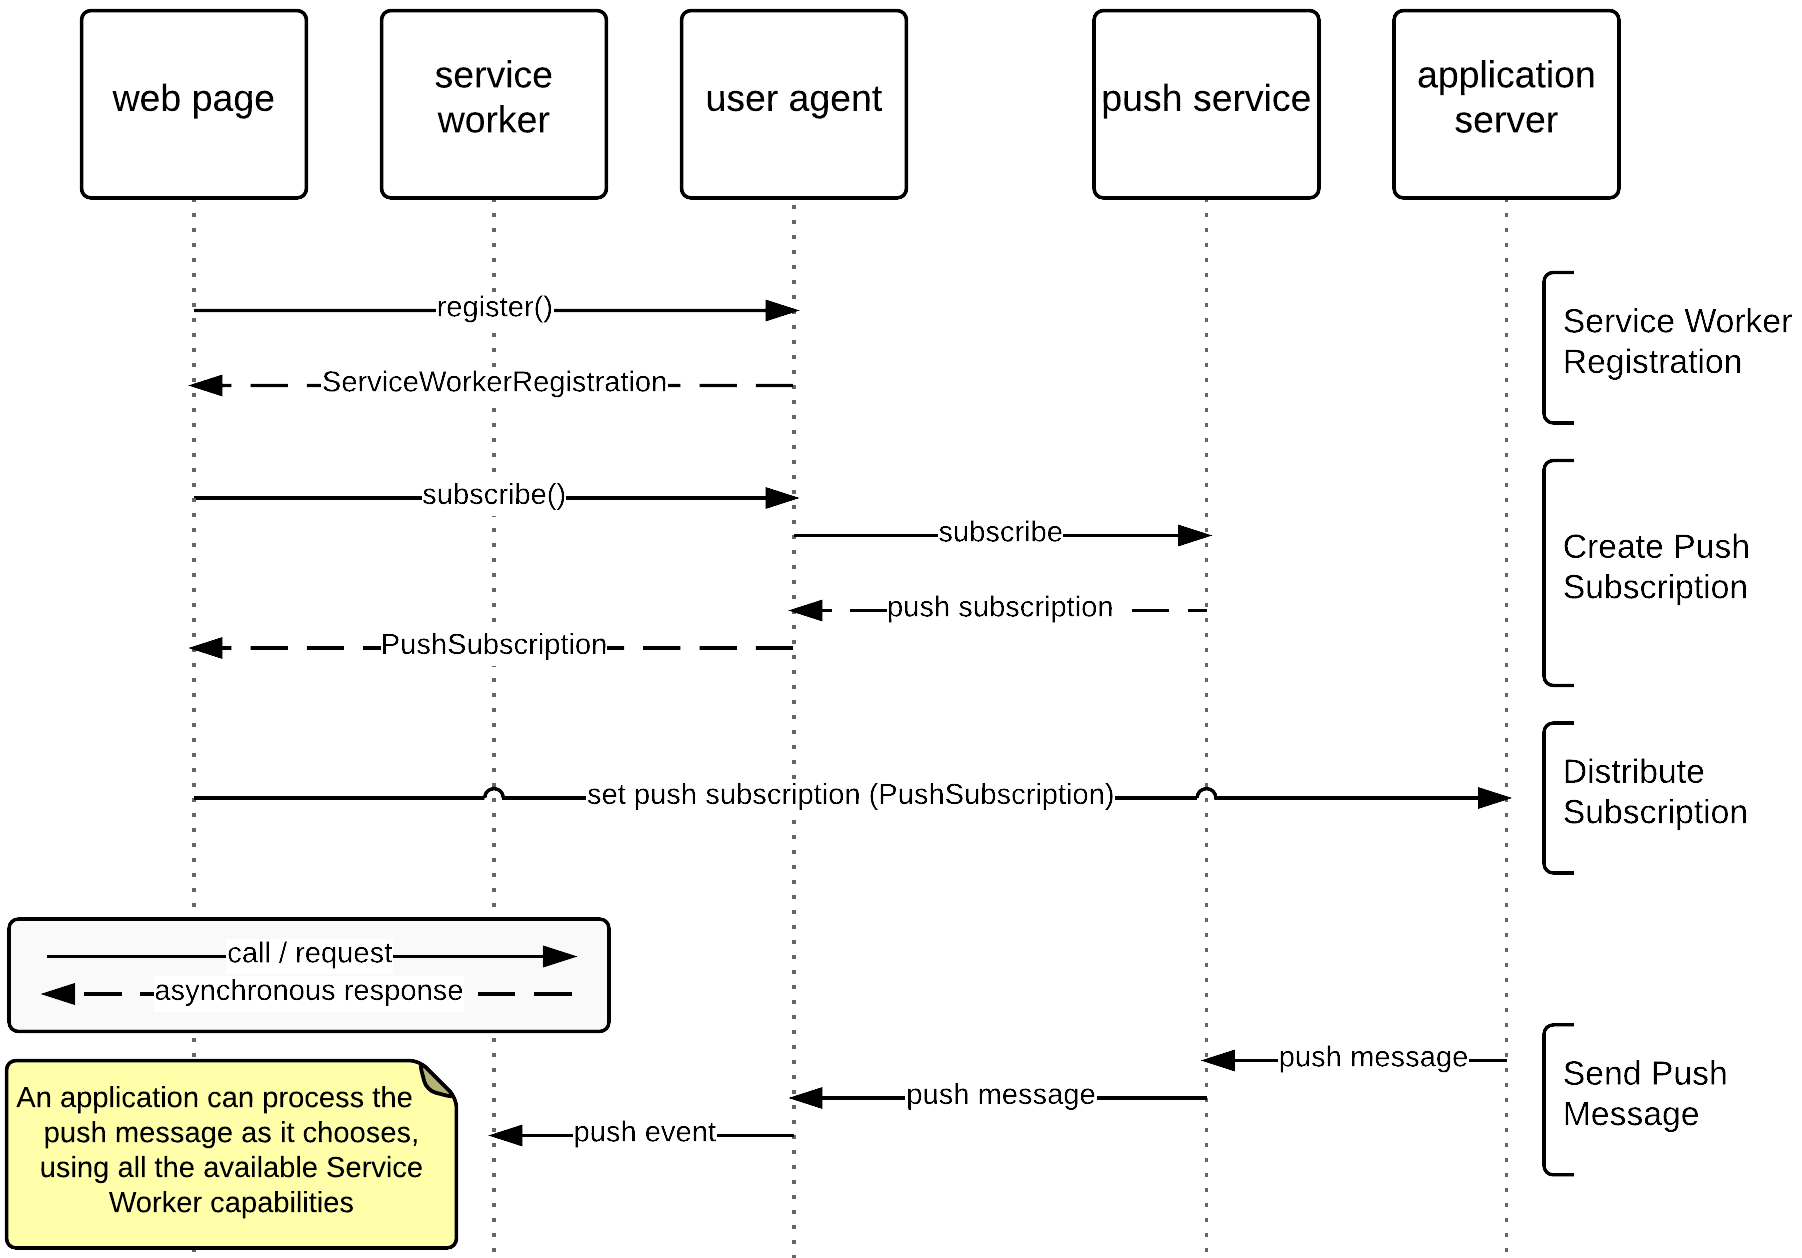
\includegraphics[width=1\textwidth]{figures/sequence_diagram_web_push.png}
 \quelle{\cite{MozillaWiki.2016}}
 \caption{Ausschnitt eines Sequenzdiagramms des Web Push Prinzips}
 \label{fig:structure_webpush}
\end{figure}

Zum besseren Verständnis der Implementierung soll zuerst das Konzept von Push umrissen werden.
Der Name Push bezieht sich darauf, dass keine Aktion vom Client vorgenommen werden muss, um diese Informationen vom Server zu erhalten.
Wie auf der rechten Seite in der Abbildung \ref{fig:structure_webpush} dargestellt, besitzt das Konzept vier Abschnitte.\\
Die erste Station betrifft die Installation des Service Workers.
Dieser wird benötigt, um Push Benachrichtigungen im Hintergrund zu erhalten, da er unabhängig von der Anwendung selbst aktiv ist und somit immer auf einen Push reagieren kann.\\
Die zweite Station findet im \textit{UserAgent}, also auf Clientseite statt.
Um Push Benachrichtungen zu ermöglichen, muss hier die Erlaubnis des Nutzers abgefragt werden.
Wird dies erlaubt, wird durch eine \textit{PushSubscription} ein Abonnement für das Gerät des aktuellen Nutzers erstellt.
Dieses Abonnement wird benötigt, um das Endgerät eindeutig zu identifizieren und somit für spätere Aktionen verfügbar zu machen.
Deshalb wird das \textit{PushSubscription}-Objekt an das Backend oder den Server versendet, um dort in einer Datenbank abgespeichert zu werden.
All dies ist Bestandteil der Push \ac{api}.\\
Die dritte Station umfasst das Auslösen einer Push Benachrichtigung in einem Backend.
Hier muss ein \ac{api}-Aufruf an einen Push Service getätigt werden, in dem alle nötigen Informationen zum Inhalt und Empfänger der Push Benachrichtigung vorhanden sind.
Dieser Aufruf wird bezeichnet als \textit{Web Push Protocol}, welches durch einen IETF\footnote{Internet Engineering Task Force. Eine Organisation, die Web-Standards entwickelt.}-Standard definiert ist.
Der Push Service ist Teil eines jeden Browsers zur Verwaltung von Push Benachrichtigungen und ist deshalb dessen Implementierung überlassen.
Jedoch ist festgelegt, dass der Service stets Anfragen in Form des \textit{Web Push Protocols} verarbeiten kann, wodurch für Entwickler die Form des Push Services irrelevant ist.\\
Die letzte Station behandelt das \textit{Push}-Event auf dem Endgerät, welches die empfangenen Daten verarbeitet und daraus eine Benachrichtigung erzeugt.
Dies wird von der Notification \ac{api} abgedeckt, welcher Zugriff auf die betriebssystemsspezifischen Benachrichtungsfunktionen besitzt.
Hierfür wird im Event die Anweisung \textit{self.registration.showNotifica\-tion(title, options)} ausgeführt.
Der Übergabeparameter \textit{title} ist dabei der Titel der Benachrichtigung und \textit{options} ein Objekt mit einer Vielzahl von Optionen wie der Text der Benachrichtigung, Aktion-Buttons, Icons und Vibrationsanweisungen.%Quelle
Im Service Worker eine Webanwendung kann auf dieses Event reagiert werden und aus den Informationen, die vom Push Service gesendet werden, eine lokale Benachrichtigung erzeugen.
Dies ist auch möglich, wenn die \ac{pwa} geschlossen ist, da der Service Worker unabhängig von der Anwendung selbst aktiv ist.
Eine aktive Internetverbindung ist jedoch unabdingbar, da der Push Service die Benachrichtigung sonst so lange einbehält, bis wieder eine Verbindung besteht.

Um den Fokus für diese Arbeit darauf zu richten, wie das Erhalten von Benachrichtigungen bei \acp{pwa} implementiert wird, wird der Backend-as-a-Service \textit{Firebase} genutzt.
Wichtig ist dabei, dass diese Funktionalität auch komplett selbst implementiert werden könnte, indem ein eigener Webserver mit beispielsweise Node.js aufgesetzt wird.
\textit{Firebase} wird von Google zur effizienten Implementierung eines Backendsystems zur Verfügung gestellt.
Speziell werden dessen Dienste \ac{fcm} und die Real Time Database genutzt.
Über dessen Konsole können einmalige sowie regelmäßige Benachrichtigungen an alle registrieren Nutzer versendet werden.
Da im Rahmen dieser Arbeit kein komplettes Management von Benachrichtigungen behandelt werden soll, werden die \textit{Keys} des \textit{PushSubscription}-Objekts lediglich in der Real Time Database abgelegt.
Daraufhin können über die \textit{Firebase} Console manuell Push Benachrichtigungen an alle \textit{Keys} versendet werden.

Damit Benachrichtigungen in der Anwendung empfangen werden können, muss erst die Erlaubnis des Nutzers erfragt werden.
Dies geschieht durch die Notification \ac{api} über den Aufruf von \textit{Notification.requestPermission()} beim Klicken des \glqq Fallzahlen abonnieren\grqq{}-Buttons.
In der asynchronen Rückgabe Funktion wird durch die \textit{messaging.getToken()}-Funktion von \textit{Firebase} ein Token für das Gerät generiert.
Im Service Worker wird dann im Falle eines Pushes vom Server im \textit{push}-Event durch die \textit{showNotification(title, body)}-Funktion eine Benachrichtigung entsendet.
\textit{Firebase} ersetzt die Nutzung des \textit{push}-Events jedoch durch seine eigene \textit{messaging.setBackgroundMessageHandler()}-Funktion, in der dasselbe durchgeführt wird.

Eine Besonderheit von der Nutzung des \ac{fcm} ist außerdem, dass dem App Manifest das Attribut \textit{gcm\_sender\_id} mit dem Wert der Sender ID hinzugefügt werden muss.
Diesen steht unter den Einstellung des \textit{Firebase}-Projekts.%???

\subparagraph{React Native App\\}
Der Prozess von Push Benachrichtigungen ist bei Native Apps ähnlich aufgebaut.
Der Push Service ist hier jedoch nicht browser- sondern betriebssystemabhängig und bezeichnet sich als \textit{Operating system push notification service (OSPNS)}.
Bei Android Geräten werden Push Benachrichtigung von dem Google Cloud Messaging (heute Firebase Cloud Messaging) verwaltet und für iOS gibt es den \ac{apn}.
Native Anwendungen benötigen wie \acp{pwa} eine Internetverbindung zum Empfangen von Push Benachrichtigungen.

Auch bei der React Native Applikation wird zur Vereinfachung des Prozesses das \ac{fcm} von \textit{Firebase} verwendet, zumal es \ac{apn} integriert.
Dafür wird die Bibliothek \glqq react-native-firebase\grqq{} genutzt, die Push Benachrichtigungen an Android und iOS ermöglicht.
In dieser Arbeit wird jedoch nur exemplarisch auf die Einrichtung von \ac{fcm} mit iOS eingegangen.
Die Native App greift nach erfolgreicher Einrichtung, die wie bei der \ac{pwa} abläuft, auf dieselbe Real Time Database zu wie die \ac{pwa}.

Push Benachrichtigungen sind eine der Funktionen, für die keine explizite Berechtigung auf Android Geräten vorhanden sein muss.
Auf der anderen Seite wird dies von der verwendeten Bibliothek nur für die iOS Implementierung benötigt.
Daher muss das Ergebnis der Funktion \textit{messaging().requestPermission()} abgefragt und dementsprechend Benachrichtigungen erlaubt oder verwehrt werden.

Auch bei nativen Anwendungen wird zwischen persistenten und nicht-persistenten Benachrichtigungen unterschieden.
Das unterscheidet sich bei der Implementierung insofern, dass das Auslösen einer Benachrichtigung nicht in der Komponente selbst mittels des \textit{messaging().onMessage()}-Funktionsaufrufs in einem \textit{useEffects} geschieht, sondern in der \textit{index.js}-Datei durch die \textit{messaging.setBackgroundMessageHandler()}-Funktion allgemein initialisiert wird.
Diese Implementierung ermöglicht nur das Empfangen von Push Benachrichtigungen, wenn die App im Hintergrund oder geschlossen ist.
\chapter{Ergebnisse und Diskussion}\label{ch:results}
Die Evaluierung der beiden Entwicklungsansätzen \ac{pwa} und Native App erfolgt nun auf Basis des in Kapitel \ref{ch:catalog} erläuterten Kriterienkatalogs.
Hierbei soll erläutert werden, ob und welche Vor- und Nachteile das Implementieren einer \ac{pwa} im Gegensatz zu einer Native App darstellt.
Außerdem wird die Frage beantwortet, ob für diesen Anwendungsfall die \ac{pwa} eine Native App ersetzen kann.

\section{Funktionalitäten}
In diesem Kapitel wird lediglich darauf eingegangen, ob Schnittstellen zur Implementierung der geforderten Funktionalitäten vorhanden sind und wie viele Möglichkeiten diese anbieten.
Die Kompatibilität der Funktionalitäten mit verschiedenen Betriebssystemen und Browsern ist Teil des nächsten Kapitels.

\subparagraph{Installierbarkeit und Aktualisierungen\\}
Lange Zeit war das Kriterium der Installierbarkeit ein signifikanter Unterschied zwischen nativen Apps und Web Applikationen.
Durch den Service Worker und dem Manifest ist dies nun möglich.
Zur Installation der programmierten \ac{pwa} wird der Link \url{https://corona-react-pwa-ba.netlify.app/} aufgerufen und das browserabhängige Vorgehen durchgeführt.
In Android ist die \glqq App installieren\grqq{}-Option unter dem Einstellungen-Symbol zu finden.
Danach ist die App auf dem Startbildschirm verfügbar und wird beim Aufrufen automatisch aktualisiert.
Hierbei fällt auf, der Nutzer automatisch durch eine Banner am unteren Bildschirmrand darauf hingewiesen wird, dass er die Anwendung herunterladen kann.
Bei Android Geräten erscheinen die Apps nach der Installation durch das generierte WebAPK zudem im App-Drawer und als App in den Einstellungen des Geräts.
Um die \ac{pwa} auf einem iOS Gerät zu installieren wird nach dem Aufrufen der App mit Safari das Teilen-Symbol geklickt und die Option \glqq Zum Home-Bildschirm\grqq{} gewählt.
Auch hier ist die Anwendung dann vom Startbildschirm aus aufrufbar und wird stets auf dem neuesten Stand des Deployments aktualisiert.\\
Bei der nativen Anwendung öffnet der Nutzer den App Store oder Play Store, navigiert zur gewünschten App, akzeptiert alle Berechtigungen und kann sie dann installieren.\\
Die Apps können dann, wie in Abbildung \ref{fig:pwa_rn_installed} abgebildet, über den Startbildschirm aufgerufen werden.

\begin{figure}[h]
\subfigure[React Native App und PWA im App-Drawer auf einem Android Gerät]{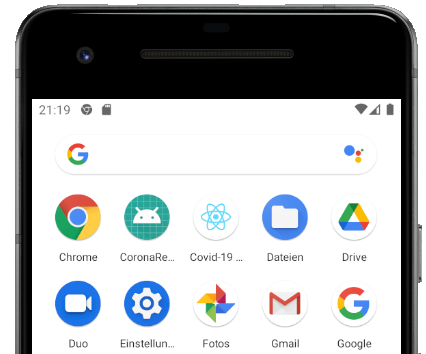
\includegraphics[width=0.5\textwidth]{figures/PWA_RN_installed.png}}
\subfigure[PWA im Startbildschirm auf einem iOS Gerät]{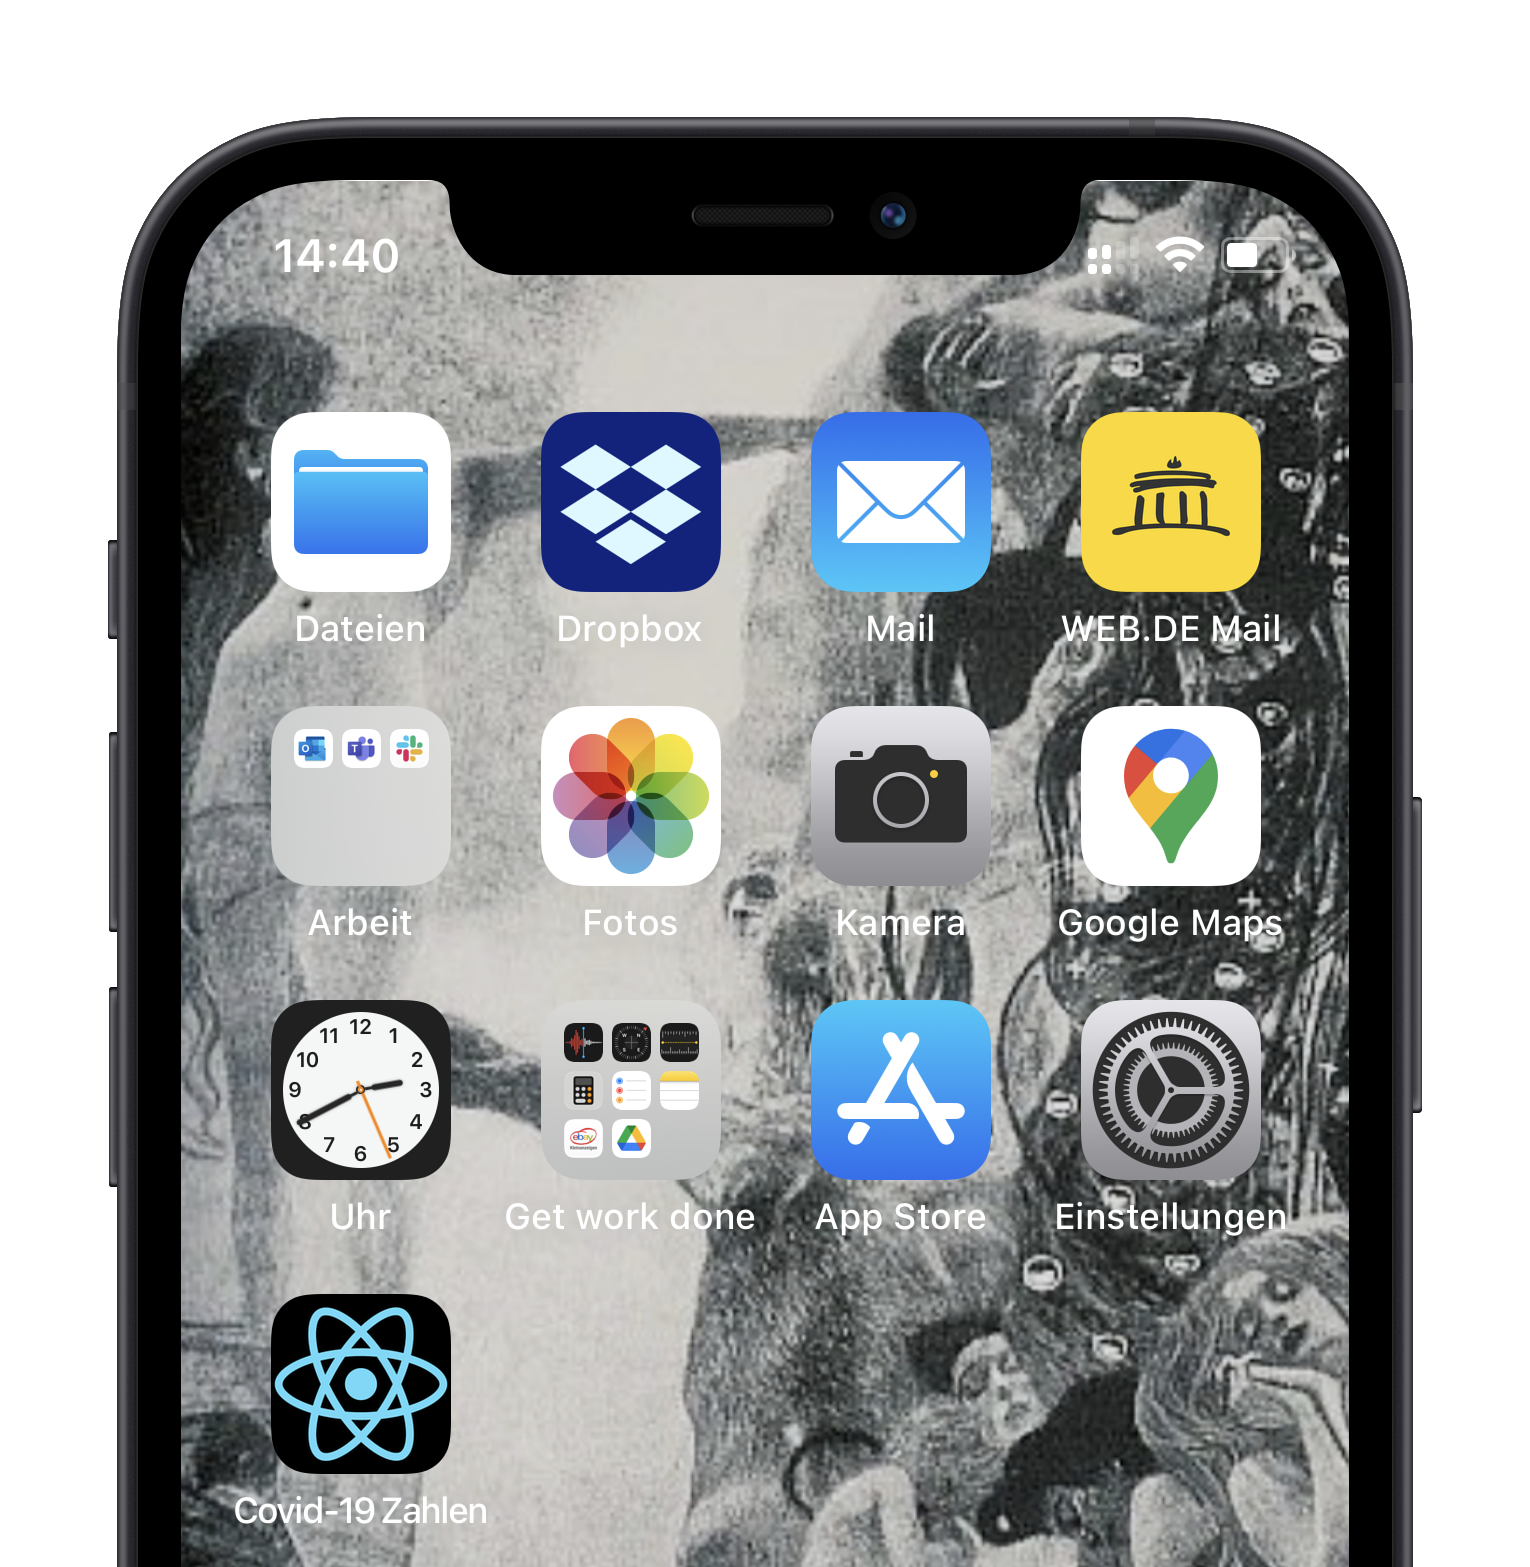
\includegraphics[width=0.5\textwidth]{figures/PWA_installed.png}}
\quelle{Eigene Darstellung}
\caption{Darstellung der installieren Apps}
\label{fig:pwa_rn_installed}
\end{figure}

Auf dem Startbildschirm sind die Anwendungen in iOS optisch nicht voneinander unterscheidbar.
Mit dem genutzten Emulator wird demgegenüber in der Chrome Version 83 durch ein kleines Browser-Symbol auf dem App-Icon deutlich, dass es sich hierbei um eine Webanwendung handelt.
In aktuelleren Browserversionen wie Chrome 91 fällt auch dieses weg, wodurch \acp{pwa} auf Android Geräten ebenfalls aussehen wie Native Apps.
Mittlerweile können auch Begrüßungsbildschirme\footnote{Wenn eine App gestartet wird, zeigt sie einige Sekunden eine Art Ladebildschirm an, bis sie bereit ist. Dabei wird meist das Logo der App und eine Hintergrundfarbe angezeigt.} für \acp{pwa} implementiert werden, wenn die Attribute \textit{name}, \textit{background\_color} und \textit{icons} im App Manifest vorhanden sind \cite{LePage.2021}.

Ein Vorteil von \acp{pwa} ist dennoch, dass sie grundsätzlich nicht installiert werden müssen.
Alle Funktionalitäten wie Standortzugriff oder Push Benachrichtigungen können aus dem Web heraus geschehen.
Native Apps hingegen können erst genutzt werden, wenn sie installiert sind.
Somit können Nutzer, deren Speicherplatz nicht für die Anwendung ausreicht, diese nicht benutzen.
Die in dieser Arbeit entwickelten Apps benötigt generell wenig Speicherplatz, da die Daten vor allem vom Server abgerufen werden, aber auch hier macht sich der Unterschied bemerkbar: die React Native App verbraucht 66.02 MB und die \ac{pwa} nur circa 0.28 MB.
Das ist darauf zurückzuführen, dass die \ac{pwa} generell weniger Ressourcen verbraucht, da es sich um gängige Webtechnologien handelt.
Gerade bei der React Native App gibt es viele Hintergrundprozesse, die Speicherplatz benötigen, um die Kommunikation zwischen Main Thread und JavaScript Thread zu ermöglichen.
Aber auch beim Vergleich zwischen klassischen, nativen Anwendungen und \ac{pwa} ist der Unterschied ähnlich: Android Apps benötigen durchschnittlich 25 MB Speicherplatz \cite{Bijlani.2021}.

Im Allgemeinen verbraucht die Installation einer \ac{pwa} außerdem weniger Datenvolumen als die einer Native App.
Ein Beispiel dafür ist die Twitter Lite \ac{pwa}, welche im Gegensatz zu den 23.5 MB der Twitter Android App lediglich 0.6 MB verbraucht \cite{Google.o.J.}.
Dies ist aber kritisch zu betrachten, da \acp{pwa} Inhalte in neuen Routen erst laden, wenn diese aufgerufen wird und somit auf langer Sicht ebenfalls so viel Datenvolumen verbrauchen können wie Native Apps.

Ferner ist es möglich, \acp{pwa} im Google Play Store zu veröffentlichen, wodurch sie einerseits durch das Web, anderseits durch den Store für Nutzer zur Verfügung stehen.
Somit können Entwickler zur Verbesserung der Auffindbarkeit der Anwendung sowohl SEO\footnote{SEO ist kurz für Suchmaschinenoptimierung} als auch ASO\footnote{Kurz für App-Store-Optimierung} durchführen.
%Da sie dennoch unabhängig von App Stores sind und entstehen für Veröffentlichung keine zusätzlichen Kosten.
%Auch bei Einnahmen der App beispielsweise durch In-App-Käufen können keine Teilbeträge verlangt werden.
Der Apple App Store unterstützt die Veröffentlichung von \acp{pwa} aktuell nicht.
Dennoch sind \acp{pwa} generell unabhängig von App Stores, da sie über das Internet erreichbar sind.
Gerade dies kann allerdings eine Schwachstelle von \acp{pwa} darstellen, da sie trotz der Veröffentlichung über HTTPS, im Gegensatz zu Native Apps keine manuelle Verifizierung zur Veröffentlichung durchlaufen müssen.

Ein entwicklungstechnischer Vorteil von \acp{pwa} gegenüber nativen Apps ist, dass sie einfacher zu verwalten sind.
Wenn es eine neue Version der Anwendung gibt, wird das Deployment durchgeführt und jeder Nutzer erhält automatisch die aktuelle Version.
Bei nativen Applikationen steckt ein Mehraufwand dahinter, da sie signiert und verifiziert werden müssen, um dann vom Nutzer aus dem jeweiligen Store aktualisiert werden zu können.\\
Diese Art von Verwaltung bei \acp{pwa} hat für die Entwickler außerdem den Vorteil, dass die Nutzer stets die neuste Version der Anwendung besitzen.
Somit ist vor allem bei langjährigen Projekten, in denen sich eventuell Schnittstellen über die Zeit ändern, Persistenz bei der Nutzung der App garantiert und es muss keine Abwärtskompatibilität implementiert werden.
Dadurch können Entwicklungs- und Wartungskosten der Anwendung reduziert werden.

\subparagraph{Offlinebetrieb\\}
Beide Anwendungen wurden auf ihre Weise offlinefähig implementiert.
Bei der \ac{pwa} bedeutet dies, dass ein Service Worker programmiert werden muss, der durch die Cache API-Anfragen abspeichert und diese bei Offlinebetrieb nutzt.
Hierbei wurden verschiedene Caching-Verfahren betrachtet und diejenige ausgewählt, die am besten zur Anwendung passt.\\
In der React Native App wurde der \textit{AsyncStorage} implementiert.
Die Daten, die durch die Netzwerkanfrage zur Verfügung stehen, werden in dessen persistente Speicher hinterlegt und genutzt, wenn keine Internetverbindung besteht.
Sie bestehen auch weiterhin, wenn die Anwendung komplett geschlossen wird.
Sobald die Verbindung wieder hergestellt wird, werden die Daten erneut aus dem Internet geladen.\\
Der Unterschied in der Implementierung des Offlinebetriebs ist, dass bei der \ac{pwa} auf fehlschlagende Netzwerkanfragen reagiert und bei der Native App der Stand der Internetverbindung abgefragt wird.
Somit werden bei der nativen Anwendung trotz der vermeintlichen \glqq Network, falling back to cache\grqq{}-Strategie nicht mehr Ressourcenanfragen gestellt als bei der \ac{pwa}.

Die Anwendungen unterscheiden sich in sofern nicht voneinander, dass beide erst nach der Installation offline verfügbar sind.
Für die \ac{pwa} bedeutet dies, dass sie zumindest einmal aufgerufen werden muss.
Denn nur wenn der Service Worker installiert und aktiviert ist, hat er die Fähigkeit, im Falle eine fehlenden Netzwerkverbindung mit zwischengespeicherten Daten zu reagieren.
Die React Native App muss ebenfalls durch das Herunterladen aus einem App Store installiert werden.
In beiden Fällen ist es außerdem möglich Vorgänge, die im Offlinebetrieb durch den Nutzer vorgenommen werden, zurückzustellen und erst auszuführen, wenn der Internetzugriff wiederhergestellt ist.
Für die \ac{pwa} bedeutet dies, dass die Background Sync \ac{api} implementiert werden muss.
%Native Anwendungen

%Ein weitere Aspekt ist, dass dem Nutzer im Offlinebetrieb bei der \ac{PWA} ähnlich wie bei Native Apps eine App Shell\footnote{•} zur Verfügung gestellt wird.
%Dies ermöglicht es, dass er zumindest eine minimale \ac{ui} nutzen und durch die Anwendung navigieren kann.
%In beiden Fällen wird auch bei Anfragen an das Netzwerk, beispielsweise für Daten aus der Datenbank, eine Internetverbindung benötigt.
%Dadurch ist der Offlinebetrieb in beiden Anwendungen gleichermaßen umgesetzt.

\subparagraph{Standortzugriff\\}
Der Standortzugriff konnte in beiden Anwendungen gleichermaßen realisiert werden.
In der \ac{pwa} wird dafür die Geolocation \ac{api} des Webs verwendet und bei der React Native App durch eine Bibliothek im Hintergrund auf die Google Location Service \ac{api} in Android und Core Location \ac{api} in iOS zugegriffen.

Ein Nachteil der \ac{pwa} bei dieser Funktionalität ist, dass durch die Geolocation \ac{api} lediglich der Zugriff auf die Koordinaten des Standorts oder das Beobachten der Position möglich ist.
Bei nativen Anwendungen gibt es in beiden Betriebssystemen inkludierte Schnittstellen (\textit{Geocoder} und \textit{CLGeocoder}), mit denen das Reverse Geocoding durchgeführt werden kann.
Dadurch entfällt bei Native Apps die Nutzung von externen Dienstleistern zur Bestimmung der Aufenthaltsort.

Außerdem ist die Geolocation \ac{api}, die in der \ac{pwa} genutzt wird, abhängig von einer aktiven Internetverbindung.
Dies ist bei Native Apps nicht der Fall, denn mobile Endgeräte können durch das verbaute GPS auf den aktuellen Standort des Nutzers zugreifen.

Zuletzt ist bei \acp{pwa} im Gegensatz zu nativen Apps die Weiterverarbeitung der Standortdaten im Sinne von beispielsweise Geofencing\footnote{Geofencing bezeichnet das Auslösen von Benachrichtigungen beim Betreten oder Verlassen von definierten Bereichen und Orten.} nicht möglich.
Ein Entwurf einer Spezifikation zur Implementierung einer solchen Funktion von 2017 ist von W3C als obsolet markiert \cite{GeofencingAPI.2017}.
% Eigentlich gibt es auch 	die watchPostion-Funktion, wieso kann die nicht für Geofencing genutzt werden?
Gerade hierfür ist darüber hinaus die Genauigkeit der Koordinaten relevant.
Ein Beispiel dafür ist das Benachrichtigen des Nutzers beim Betreten unterschiedlicher Räume in einer Wohnung, ferner aber auch das Bestimmen des Standorts eines verlorengegangenen Geräts.
Für die implementierte App ist die Genauigkeit der Koordinaten nicht von Bedeutung, da lediglich die Stadt ermittelt werden soll, in welcher der Nutzer der App sich befindet.
Beim Testen wird jedoch deutlich, dass die Koordinaten, wie in Abbildung \ref{fig:comparison_geoloc}, exakt übereinstimmen.

\begin{figure}[h]
\subfigure[Standortbestimmung PWA]{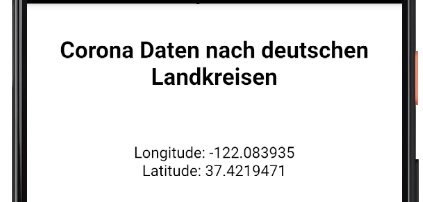
\includegraphics[width=0.49\textwidth]{figures/Geoloc_PWA.png}}
\subfigure[Standortbestimmung React Native App]{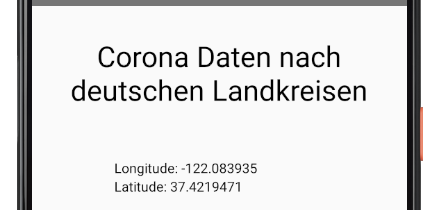
\includegraphics[width=0.49\textwidth]{figures/Geoloc_RNA.png}}
\quelle{Eigene Darstellung}
\caption{Darstellung der bestimmten Koordinaten}
\label{fig:comparison_geoloc}
\end{figure}
%Paper FULLTEXT01.pdf
%Aus technischer Sicht außerdem interessant, dass die Geolocation API, die in der PWA genutzt wird, eine bessere Performance unter Beweis stellt als der Standortzugriff einer Android App.
%Wieso? Beweise?

\subparagraph{Kontaktzugriff\\}
Diese Funktionalität wurde mit der Contact Picker API implementiert.
Durch sie ist es möglich aus den vorhandenen Kontakten des Geräts einen Kontakt auszuwählen und auf dessen Daten, darunter auch die Adresse, zuzugreifen.\\
Mit React Native gibt es keine Probleme mit der Umsetzung.
Durch das Einbinden einer \textit{Bridge} mittels einer externen Bibliothek konnte diese Funktionalität programmiert werden.

Der Zugriff auf eine grundlegende Schnittstelle wie der Kontaktliste ist für native Anwendungen selbstverständlich.
Dabei ist sowohl das Lesen als auch die Erstellung und Modifikation von Kontakten möglich.
Die Contact Picker \ac{api} bietet hingegen aktuell nur das Lesen der Kontaktliste an.
Das geschieht in einer browsereigenen Darstellungform, die in \ref{fig:contact_picker_ui} für den Chrome Browser abgebildet ist.
Entwürfe für das Erweitern der Funktionalität dieser \ac{api} liegen aktuell nicht vor.

\begin{figure}[h]
 \centering
 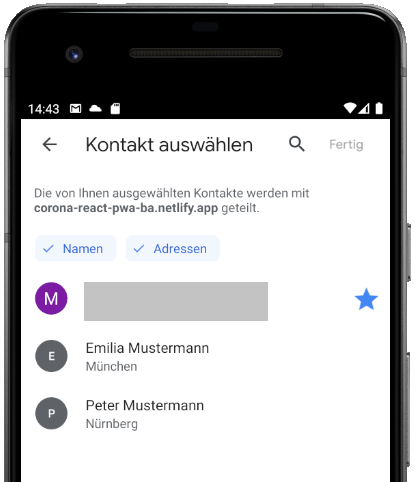
\includegraphics[width=0.6\textwidth]{figures/contact_picker_ui.png}
  \quelle{Eigene Darstellung}
 \caption{Benutzeroberfläche der Contact Picker \ac{api} in Chrome}
 \label{fig:contact_picker_ui}
\end{figure}

\subparagraph{Benachrichtigungen\\}
Optisch lassen sich die Benachrichtigungen von \acp{pwa}, wie in Abbildung \ref{fig:pushnotifications_comparison} zu erkennen ist, nicht von denen von Native Apps unterscheiden.
Dies ist damit zu erklären, dass in beiden Fällen auf die betriebssystemspezifische Benachrichtigungsfunktion zugegriffen wird.
Auch im Aspekt Aktionen bieten die zwei Apps dieselben Möglichkeiten.
Bei beiden ist es möglich, Aktionen zu definieren, die von der Benachrichtigungszeile aus getätigt werden können.
Das betrifft beispielsweise das Beantworten einer Nachricht oder das Löschen einer E-Mail.

\begin{figure}[h]
 \centering
 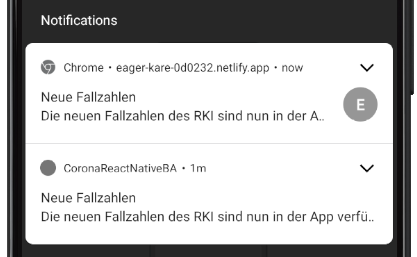
\includegraphics[width=0.6\textwidth]{figures/Push_notifications.png}
  \quelle{Eigene Darstellung}
 \caption{Vergleich Benachrichtigungen PWA (oben) und React Native App (unten)}
 \label{fig:pushnotifications_comparison}
\end{figure}

Dennoch wird bei den Benachrichtigungen eine weitere Schwachstelle von \acp{pwa} deutlich.
Der Safari Browser erlaubt auf mobilen Endgeräten aktuell weder persistente noch nicht-persistente Benachrichtigungen von Webanwendungen.
Laut \textit{caniuse} implementiert der Safari Browser eine eigene Version der Push API, die jedoch nicht für Safari auf iOS verfügbar ist \cite{caniuse.com.2021}.
%Woran liegt es, dass es von Apple noch nicht unterstützt wird sich das in Zukunft ändern?

\subparagraph{Zusammenfassung\\}
Generell besitzt das Web alle Schnittstellen, um die im Kapitel \ref{ch:catalog} definierten Funktionalität umzusetzen.
Bei der Implementierung der Funktionalitäten wird dennoch deutlich, dass \acp{pwa} nicht beliebige native Schnittstellen aufrufen können, sondern lediglich Webschnittstellen nutzen.
Diese befinden sich noch im Aufbau und sind deshalb nicht umfassend, als experimentell markiert, nicht von jedem Browser unterstützt oder existieren nicht.
Das hat bei der Verwendung jener Schnittstellen zufolge, dass sich im Laufe der Zeit Schnittstellen verändern, ersetzt oder sogar entfernt werden.
Deshalb sollten diese mit Vorsicht genutzt werden.
Beispielsweise ist das App Manifest aktuell vom \textit{W3C} als experimentell gekennzeichnet und die Contact Picker \ac{api} noch ein inoffizieller Entwurf \cite{MDNcontributors.d}\cite{Beverloo.2021}.

%Bezogen auf die in dieser Arbeit implementierte App kann rein vom Funktionsumfang die \ac{pwa} eine Native App ersetzen.

%Web App Gap
%Project Fugu

%Großes Problem bei PWAs allgemein ist die fehlenden Unterstützung von Apple. Das macht aber auch Sinn, da sie viel daran verdienen, dass leute eine Lizenz für jeden Anwendung und deren In-App-Verläufe zahlen müssen

%PWA kommt nicht gut mit der großen Datenmengen zurecht, Werte wie Largest Contentful Paint und Total Blocking Time sind nicht gut

%React Native hat eine Code Push Funktionalität, die es erlaubt neue Versionen des Codes zu veröffentlichen ohne dass der Nutzer eine Aktualisierung durchführen muss.
%Das ist gut für den Nutzer, aber kann Probleme bei der Veröffentlichung im App Store mitbringen, weil dort normalerweise jede Code Änderung verifiziert werden muss.

\section{Kompatibilität mit verschiedenen Betriebssystemen} 
Durch das Testen der Apps auf jeweils einem iOS und einem Android Smartphone soll nun die Kompatibilität der beiden Anwendungen überprüft werden.
Hierfür wird ein Apple IPhone 12 mit iOS 14 und ein Huwaei P10 Lite mit Android 10 verwendet.
Die Native App wird mit einem Google Pixel 4 Emulator mit Android 11 getestet.

\subparagraph{Progressive Web App\\}
Die \ac{pwa} ist unter dem Link \url{https://corona-react-pwa-ba.netlify.app/} erreichbar.
Hierdurch kann sie mit jedem Browser eines internetfähigem Geräts erreicht werden, wodurch sie größtenteils betriebssystemunabhängig sind.
Falls ein Browser dennoch gewisse Funktionalitäten der \ac{pwa} nicht unterstützt, wird durch den Ansatz des Progressive Enhancements sichergestellt, dass die Seite zumindest die aktuellen Corona-Daten darstellt und diese nach dem Namen des Landkreises filtern kann.

In der Tabelle \ref{fig:compability_android} sind die Ergebnisse des Testens aufgelistet.
In Klammern dahinter steht zusätzlich jeweils die Browserversion, ab dem laut \textit{MDN Web Docs} diese Funktionalität unterstützt wird.
Bei der Verwendung eines Android Geräts können die meisten Funktionen genutzt werden, lediglich der Kontaktzugriff entfällt auf dem Firefox Webbrowser.
Für die Installierbarkeit mit Opera gibt es von \textit{MDN Web Docs} keine Angaben über die Browserversion.
Die Verifizierung konnte jedoch beim Testen mit der Opera Version 64 nachgewiesen werden.
Über die Nutzung der \ac{pwa} auf einem Android Gerät mit dem Safari Browser konnten keine Daten erhoben werden, da die Safari App im Google Play Store nicht zu Verfügung steht.

\begin{table}[h]
\centering
\caption{Kompatibilität der Progressive Web App mit verschiedenen Browsern auf einem Android Gerät}
\begin{tabular}[h]{|c||c|c|c|c|}
\hline
\textbf{Funktionalität} & \multicolumn{4}{|c|}{\textbf{Browser auf Android Gerät}} \\
\hline
 & Chrome & Firefox & Opera & Safari \\
\hline
Installierbarkeit & ja (39) & ja (53) & ja (\kA) & - \\
\hline
Offlinebetrieb & ja (40) & ja (39) & ja (27) & - \\
\hline
Standortzugriff & ja (18) & ja (4) & ja (11) & - \\
\hline
Kontaktzugriff & ja (80) & nein & ja (57) & - \\
\hline
Benachrichtigung & ja (42) & ja (44) & ja (37) & - \\
\hline
\end{tabular}
\label{fig:compability_android}
\end{table}

Die Tabelle \ref{fig:compability_ios} zeigt die Ergebnisse der Kompatibilität bei Nutzung eines iOS Geräts.
Hierbei wird deutlich, dass die \ac{pwa}, wenn sie im Chrome, Opera oder Firefox Webbrowser aufgerufen wird, nicht die Funktionalität der Installierbarkeit unterstützt.
Das ist damit zu begründen, dass iOS diese Browser mit WebKit rendert, statt mit den eigenen HTML-Renderern (\zB Blink für Chrome).
%Denn jede iOS App muss laut Punkt 2.5.6 der Apple App Store Review Guidelines als Engine WebKit nutzen \cite{Apple.07.06.2021}.
%einfach nicht supported https://support.google.com/chrome/answer/9658361?hl=en&co=GENIE.Platform%3DiOS
Ferner fehlt die Unterstützung des Kontaktzugriffs und Push Benachrichtigungen.
Ersteres ist seit iOS Version 14.15 und Safari 14.1 auch bei iOS Gerät als experimentelle Funktion verfügbar, jedoch ist das nur auf die Kontaktdaten \textit{name}, \textit{email} und \textit{tel} (Telefonnummer) beschränkt \cite{Firtman.2021}.
Dennoch zeigt dies, dass sich Apple einer Implementierung moderner Browserschnittstellen für den Safari Browser annähert.
Über eine Umsetzung von Push Benachrichtigungen auf mobilen Endgeräten gibt es aktuell keine Auskünfte \cite{Firtman.2021}.

\begin{table}[h]
\centering
\caption{Kompatibilität der Progressive Web App mit verschiedenen Browsern auf einem iOS Gerät}
\begin{tabular}[h]{|c||c|c|c|c|}
\hline
\textbf{Funktionalität} & \multicolumn{4}{|c|}{\textbf{Browser auf iOS Gerät}} \\
\hline
 & Chrome & Firefox & Opera & Safari \\
\hline
Installierbarkeit & nein & nein & nein & ja (11.3) \\
\hline
Offlinebetrieb & ja (40) & ja (44) & ja (27) & ja (11.3) \\
\hline
Standortzugriff & ja (18) & ja (4) & ja (11) & ja (3) \\
\hline
Kontaktzugriff & nein & nein & nein & teilweise (14.7) \\
\hline
Benachrichtigung & nein & nein & nein & nein \\
\hline
\end{tabular}
\label{fig:compability_ios}
\end{table}

Neben den teilweise fehlenden Funktionalitäten in bestimmen Browsern und Browserversionen ist weiteres Problem von \acp{pwa}, dass einige der verwendeten Schnittstellen als experimentell gekennzeichnet sind.
Das hat bei deren Verwendung jener Schnittstellen zufolge, dass sich im Laufe der Zeit Schnittstellen verändern oder sogar ersetzt werden.
Diese Unsicherheit kann für einige Projekte ein ausschlaggebender Faktor gegen die Implementierung einer \ac{pwa} sein.
Aktuell betrifft das \acp{api} und Technologien wie das App Manifest, die Push \ac{api} und die Funktionen der Contact Picker \ac{api} \cite{MDNcontributors.d,MDNcontributors.2021,MDNcontributors.22.06.2021}.

\subparagraph{React Native\\}
Die React Native Android App kann nach dem Ausführen des Befehls \glqq npx react-native start\grqq{} und \glqq npx react-native run-android\grqq{} auf einem Emulator oder einem angeschlossenen Android Gerät genutzt werden.
Für die Nutzung auf einem iOS Gerät muss der korrespondieren Befehl \glqq npx react-native run-ios\grqq{} auf einem Mac-PC durchgeführt werden.
Dadurch, dass bei der Entwicklung der Anwendung kein Mac-PC zur Verfügung stand, konnte nicht zeitgleich geprüft werden, ob die React Native Anwendung alle Funktionalitäten auch in iOS unterstützt.
Es wird dennoch davon ausgegangen, dass alle geforderten Funktionen wie bei der Android App funktionieren, weil alle verwendeten Bibliotheken als kompatibel mit Android und iOS gekennzeichnet sind.%Quelle?

%Generell gilt jedoch, dass native Anwendungen nur auf dem Betriebssystem installiert werden können, für das sie programmiert wurden.
%Das heißt, dass eine Native App beim Faktor Kompatibilität mit verschiedenen Betriebssystemen nicht vergleichbar ist mit einer \ac{pwa}.

\subparagraph{Zusammenfassung\\}
Die Unterstützung von \acp{pwa} auf Apple Geräten hat sich seit iOS 11.3 verbessert, da mit dieser Version Schnittstellen wie der Service Worker, das App Manifest oder xx verfügbar sind.% ????
Allerdings ist es, wie bereits im Kapitel \ref{ch:implementation} beschrieben, aktuell nicht möglich, Push Benachrichtigungen auf einem iOS Smartphone zu erhalten oder den Zugriff auf die Kontakte zu ermöglichen.%Quelle
Das ist ein großer Nachteil von \acp{pwa}, da 26,34 Prozent des Marktanteils somit nicht bedient werden können \cite{ODea.2021}.
Außerdem geht damit ein ausschlaggebender Faktor zur laufenden Interaktion mit den Nutzern verloren.
Auch in naher Zukunft arbeitet Apple aktiv nicht an einer Implementation dieser Funktionalität. %Quelle, warum

Rein von der Auswahl der verschiedenen Betriebssysteme, auf denen eine \ac{pwa} aufgerufen werden kann, hat eine \ac{pwa} mehr Reichweite.
Da die Kompatibilität jedoch lückenhaft ist, kann dies nicht als Vorteil der \ac{pwa} gesehen werden.
Vor allem die fehlende Unterstützung von iOS Geräten spricht gegen deren Etablierung.
Eine React Native App verspricht mehr Kompatibilität als eine Native App, jedoch konnte auch dies nicht bestätigt werden, da die iOS App in diesem Falle bereits beim Aufsetzen der Entwicklungsumgebung gescheitert ist.
Bei einer Ausstattung mit einem Mac-Computer wäre dies weniger problematisch, denn dort ist eine zeitgleiche Entwicklung für iOS und Android möglich.
Dies trifft ebenso für die Nutzung des Expo Frameworks zu, da dadurch auch auf einem Windows Computer eine auf beiden Betriebssystemen lauffähige App entwickelt werden kann.
Native Apps selbst sind nach wie vor betriebssystemabhängig, wodurch sich die Kompatibilität mit verschiedenen Betriebssystemen erübrigt.

Zusammenfassend bedeutet dies dennoch, dass \acp{pwa} im Bezug auf Kompatibilität mit verschiedenen Betriebssystemen Native Apps voraus sind, da sie generell auf beiden betrachteten Betriebssystemen lauffähig sind.
Die Unterstützung einzelner Funktionalitäten ist wiederum eine Schwachstelle von \acp{pwa}, da manche nicht auf iOS Geräten existieren.
Plattformunabhängige Apps hingegen bieten -- wenn eine geeignete Entwicklungsumgebung zur Verfügung steht -- für die geforderten Funktionalitäten am meisten Kompatibilität mit verschiedenen Betriebssystemen.

\section{Entwicklungsaufwand}
Zur Bestimmung des Entwicklungsaufwand wurde einerseits die Dauer der Recherche gemessen und andererseits die reine Implementierungsdauer.
Ersteres umfasst dabei die Einarbeitung in Technologien und das Studieren der Spezifikationen, die für die Funktionalitäten benötigt werden.
Die Anwendungen wurden mit einem soliden Grundwissen in HTML, CSS und JavaScript entwickelt.
Tiefgehende Kenntnisse der Bibliothek und des Frameworks waren vor der Programmierung der Apps nicht vorhanden.
In der Tabelle \ref{fig:outlay_comparison} ist die Auflistung der Aufwände dargestellt.

\begin{table}[h]
\centering
\caption{Entwicklungsaufwand der beiden Anwendungen}
\begin{tabular}[h]{|p{3cm}||c|c|c|c|}
\hline
\textbf{Funktionalitäten} & \multicolumn{2}{|c|}{\textbf{Recherche}} &\multicolumn{2}{c|}{\textbf{Implementierung}} \\
\hline
 & PWA & Native App & PWA & Native App \\
\hline
\makecell{Einrichten der\\Entwicklungs-\\umgebung} & 60 min & 240 min & 25 min & 60 min \\
\hline
Installierbarkeit & 30 min & 60 min & 30 min & 15 min \\
\hline
Offlinebetrieb & 100 min & 40 min & 45 min & 30 min \\
\hline
Standortzugriff & 30 min & 45 min & 15 min & 30 min \\
\hline
Kontaktzugriff & 60 min & 45 min & 45 min & 30 min \\
\hline
Benachrichtigung & 300 min & 250 min & 120 min & 200 min \\
\hline
\hline
Gesamt & 580 min & 680 min & 280 min & 395 min \\
\hline
\end{tabular}
\label{fig:outlay_comparison}
\end{table}

Beim Einrichten der Entwicklungsumgebung konnten in beiden Fällen Toolchains zur Beschleunigung des Prozesses genutzt werden.
Dennoch hat dies bei React Native mehr Zeit beansprucht als bei dem Aufsetzen der \ac{pwa}, weil neben der Installation der CLI weitere Vorkehrungen zur Einrichtung der Umgebungsentwicklung getätigt werden mussten.
Das betrifft beispielsweise das Konfigurieren von Android Studio oder das Aufsetzen eines \ac{avd}.
Bei der \ac{pwa} musste lediglich der Befehl \glqq npx create-react-app corona-react-pwa-ba\grqq{}\footnote{Letzteres ist der Name der Anwendung und kann frei gewählt werden} ausgeführt werden und ein vollständiges Setup zum Entwickeln einer Single Page Application ist erstellt.
Diese konnte dann sofort mit Webpack auf einem Webserver gestartet und weiterentwickelt werden.\\
Die Installierbarkeit hat bei \acp{pwa} circa doppelt so lange benötigt, weil konkrete Implementierungen vorgenommen werden mussten, um dies hierbei zu ermöglichen.
Beispielsweise musste das App Manifest erstellt und Icons zur Verfügung gestellt werden.
Native Apps sind generell installierbar, sie müssen lediglich zur Veröffentlichung in einem App Store signiert werden.\\
Das Ermöglichen des Offlinebetriebs hat bei der \ac{pwa} mehr Zeit beansprucht, da hier die verschiedenen Arten des Cachings der Daten betrachtet und ausgewählt werden mussten.
Für die Umsetzung in der Native App wurde der gängige \textit{AsyncStorage} in Kombination mit der React Native Bibliothek \textit{NetInfo} gewählt.\\
Das Ermöglichen des Standortabfrage hat in beiden Anwendungen ungefähr gleich viel Zeit in Anspruch genommen.\\
Die Recherche für die Implementierung des Kontaktzugriffs benötigte in der \ac{pwa} länger, da diese Funktion erst seit Chrome 80 auf Android zu Verfügung steht und somit wenig Literatur vorhanden ist \cite{Beverloo.2021}.
Auch die Programmierung selbst ist aufwendiger, da der Kontaktzugriff nur mit dem Emulator über \ac{https} und nicht mit \textit{localhost} möglich ist, weshalb die \ac{pwa} stets deployt werden musste.\\
Die Benachrichtigungen sind bei React Native mit mehr Aufwand verbunden, da die Kompatibilität auf beiden betrachteten Betriebssystemen gewährleistet werden muss.
Jedoch sind die Zeiten auch hier mit Vorsicht zu betrachten, da die \ac{pwa} auf iOS generell keine Benachrichtigungsfunktion zur Verfügung stellen kann und somit möglicherweise nötige Polyfills beim Entwicklungsaufwand entfallen.\\
Der Gesamtaufwand für die Recherche und Implementierung der \ac{pwa} beträgt somit circa 16 Stunden (850 min) und fast 18 Stunden (1075 min) für die React Native App. 

Insgesamt wird deutlich, dass für die Einfindung und Implementierung der React Native App im Gegensatz zur \ac{pwa} mehr Zeit beansprucht wurde, obwohl Teile des Codes wiederverwendet werden konnten.
Besonders ausschlaggebend war dabei die Einarbeitung in die Technologien zur plattformunabhängigen Implementierung.
Denn zur Entwicklung mit React Native muss einerseits React Native verstanden und anderseits Kenntnisse in nativer Programmierung aufgebaut werden.
Dies betrifft beispielsweise den Aufbau nativer Anwendungen und die betriebssystemspezifischen Programmiersprachen.\\
Hierbei muss außerdem beachtet werden, dass in dieser Arbeit aufgrund der Tatsache, dass kein Mac-Computer zur Entwicklung der Native App für iOS vorhanden war.
Das wirkt sich insofern auf den Entwicklungsaufwand aus, dass theoretisch für die Implementierung mehr Zeit in Anspruch genommen werden muss, weil eventuell auftretende Schwierigkeiten behoben werden müssen.
Zum Beispiel ist die Einrichtung von Push Benachrichtigungen für iOS mit \textit{Firebase} ein hinzukommender Aufwand, da dies separat von der Android Version gemacht werden muss.
Somit steigt der tatsächliche Entwicklungsaufwand der React Native App zusätzlich.

Die Ergebnisse der Entwicklungsaufwände sind nach Meinung des Autors kritisch zu betrachten, da bei der Programmierung der \ac{pwa} deutlich weniger fremder Code verwendet wurde als für die React Native App.
Hier ist es nämlich Teil des Arbeitsablaufs, sich vor-implementierten Bibliotheken zu bedienen, da oftmals \textit{Bridges} für gängige Funktionalitäten bereits existieren.
Würden diese nicht verwendet werden, wäre der Entwickungsaufwand der React Native App deutlich höher.
Auch für die \ac{pwa} könnten Bibliotheken und Werkzeuge genutzt werden, wie etwa das bereits erwähnte Tool \glqq Workbox\grqq{} von Google.
Dennoch spricht es für die \ac{pwa}, dass keine Abhängigkeit von anderen Bibliotheken benötigt werden, sondern die Funktionalität lediglich durch moderne Schnittstellen geschieht, die das Web anbietet.
Eine Native mit Java oder Swift implementierte App besitzt ebenso weniger Abhängigkeiten als die React Native App, da sie auf die nativen Schnittstellen der Betriebssysteme zugreifen.
Diese Abhängigkeit ist also nur eine Besonderheit von React Native Apps.

Außerdem ist an dieser Stelle anzumerken, dass der Entwicklungsaufwand einer mit React Native entwickelten App nicht gleichzusetzen ist mit einer tatsächlich nativen App.
Diese benötigt für dasselbe Ergebnis zwei Implementierungen, eine für Android und eine für iOS.
Dadurch kann sich der Recherche- und Entwicklungsaufwand verdoppeln, zumal auch eine Einarbeitung in zwei verschiedene Programmiersprachen und Entwicklungsumgebungen stattfinden muss.

Ein großer Nachteil der Entwicklung mit React Native ist, dass aktuell nicht komplett plattformunabhängig programmiert werden kann.
So ist ein Mac-Computer die Voraussetzung zur Implementierung von nativen iOS Komponenten in einer React Native Anwendungen.
Das betrifft auch die Ansprache von spezifischen Schnittstellen wie Touch oder Face ID, Bluetooth und selbst Batterieverbrauch von iOS Geräten. %Quelle
Theoretisch können auch externe Dienstleister diese Teile der Implementierung übernehmen, jedoch bringt das weitere Entwicklungskosten und eine höheren Managementbedarf.
Im Gegensatz dazu sind \acp{pwa} in der Entwicklung grundlegend unabhängig, da es sich dabei um normale Webanwendungen handelt, welche keine spezifische Entwicklungsumgebung benötigen.

Ferner muss betont werden, dass es sich bei React Native App trotz der Programmierung großer Teile in JavaScript im Endeffekt um zwei Technologien handelt, die der Entwickler beherrschen muss.
Einerseits JavaScript für das Implementieren einer Anwendung mit React, andererseits das Wissen über native Entwicklung, Schnittstellen und betriebssystemabhängige Programmiersprachen, um gegebenenfalls plattformspezifischen Code zu ergänzen.
Das wirkt sich insofern auf den Entwicklungsaufwand aus, dass JavaScript-Entwickler, die keine noch Erfahrungen mit nativer App-Entwicklung haben, mehr Zeit für die Einarbeitung in die Thematik benötigen.

\begin{figure}
\subfigure[React App Texteingabe Implementierung]{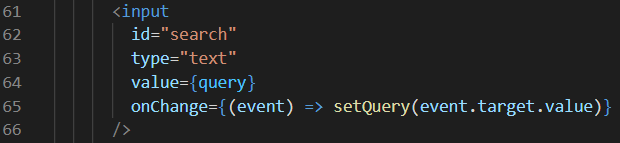
\includegraphics[width=0.49\textwidth]{figures/Input_R.png}}
\subfigure[React Native Texteingabe Implementierung]{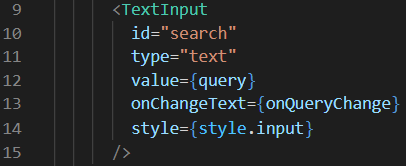
\includegraphics[width=0.49\textwidth]{figures/Input_RN.png}}
\quelle{Eigene Darstellung}
\caption{Vergleich Implementierung React PWA und React Native App}
\label{fig:textinputComparison}
\end{figure}

Ein besonderer Vorteil dieser Konstellation von Technologien ist jedoch, dass Teile der Logik und Aufteilung der Komponenten aus der React Web App in die React Native App übernommen werden können und somit Zeit gespart wird.
Ein Beispiel dafür ist in der Abbildung \ref{fig:textinputComparison} verdeutlicht.
Hieran wird sichtbar, dass in vielen Fällen die Syntax nur abgeändert werden muss, um die React Version der Implementierung in React Native zu übertragen.
Das ist vor allem dann eine Option, wenn im Laufe des Projekts klar wird, dass die Funktionalitäten, die \acp{pwa} aktuell anbieten, nicht ausreichen.
Diese Art von flexibler Entwicklung bieten native Anwendungen grundsätzlich nicht.

\section{Diskussion}
In der Tabelle \ref{fig:discussion_impl} soll nun auf Grundlage der dargestellten Argumente die Erfüllung der einzelnen Kriterien in Form von Punkten bewertet werden.
Auf eine Gewichtung der Kriterien wurde durch den Anwendungsfall bewusst verzichtet.% Warum?
Die Bewertung beruht auf folgenden Definitionen:
\begin{itemize}
\item 0 Punkte: Das Kriterium konnte nicht erfüllt werden.
\item 1 Punkt: Das Kriterium konnte teilweise erfüllt werden.
\item 2 Punkte: Das Kriterium konnte vollkommen erfüllt werden.
\end{itemize}

\begin{table}[h]
\centering
\caption{Nutzwertanalyse der beiden implementierten Anwendungen}
\begin{tabular}[h]{|c||c|c|}
\hline
\textbf{Kriterium} & \textbf{PWA} & \textbf{Native App} \\
\hline
Funktionalität & 2  & 2 \\
\hline
\makecell{Kompatibilität \\mit vers. \\Betriebssystemen}  & 1  & 2 \\
\hline
Entwicklungsaufwand  & 2  & 1 \\
\hline
\hline
Summe & 5  & 5 \\
\hline
\end{tabular}
\label{fig:discussion_impl}
\end{table}

Beim Kriterium der Funktionalität erreichen beide Apps für den definierten Anwendungsfall die maximale Punktzahl, da alle geforderten Funktionen mit beiden Technologien umgesetzt werden können.
Die Kompatibilität mit verschiedenen Betriebssystemen war bei \acp{pwa} nicht vollkommen gegeben, da Safari, wie bereits erläutert, einige Funktionalitäten nicht unterstützt.
Das Kriterium des Entwicklungsaufwands erfüllt die \ac{pwa} wiederum besser, weil sowohl die Recherche- als auch die Implementierungszeit geringer war als bei der React Native App.
Deshalb erhält die \ac{pwa} in diesem Aspekt eine höhere Punktzahl.\\
Das Ergebnis zeigt, dass in diesem Anwendungsfall die Native App durch eine \ac{pwa} ersetzt werden kann.

Nun sollen in einer weiteren Tabelle \ref{fig:discussion_gen} die Erfüllung der Kriterien durch die zwei Technologien im Allgemeinen betrachtet werden.
Hierbei wurde zusätzlich eine tatsächlich Native App für den Vergleich aufgenommen, denn diese unterscheidet sich insofern, dass nicht kompatibel mit verschiedenen Betriebssystemen ist.
Auch der Entwicklungsaufwand ist höher, denn um dasselbe Ergebnis zu erreichen wie bei einer PWA oder React Native App muss für jedes Betriebssystem eine eigene App mit der jeweiligen Entwicklungsumgebung entwickelt werden.
Im Gegensatz zur vorherigen Tabelle wird deutlich, dass \acp{pwa} weniger Funktionalitäten unterstützen als React Native oder Native Apps.
Beispielsweise betrifft das in dieser Arbeit nicht behandelte Funktionen wie das Geofencing oder die User Idle Detection\footnote{Das Erkennen, ob der Nutzer den Bildschirm aktiv betrachtet.} \cite{AppBar.2021}.
Die anderen Kriterien sind bei der \ac{pwa} und React Native App gleichermaßen erfüllt.\\

\begin{table}[h]
\centering
\caption{Nutzwertanalyse der beiden Technologien im Allgemeinen}
\begin{tabular}[h]{|c||c|c|c|}
\hline
\textbf{Kriterium} & \textbf{PWA} & \textbf{React Native App} & \textbf{Native App} \\
\hline
Funktionalität & 1  & 2 & 2 \\
\hline
\makecell{Kompatibilität \\mit vers. \\Betriebssystemen}  & 1  & 2 & 0 \\
\hline
Entwicklungsaufwand  & 2  & 1 & 0 \\
\hline
\hline
Summe & 4  & 5 & 2 \\
\hline
\end{tabular}
\label{fig:discussion_gen}
\end{table}

Anhand des Vergleichs der beiden Nutzwertanalysen wird klar, dass \acp{pwa} nicht allgemein als Ersatz zu nativen Anwendungen gesehen werden können.
Die Ergebnisse legen zudem zusammenfassend nahe, dass eine Entscheidung für eine der beiden Implementationen abhängig von den Anforderungen an die zu entwickelnde  getroffen werden sollte.
\chapter{Fazit und Ausblick}\label{ch:summary}
%Klärung der wissenschaftlichen Frage, Bezug auf Einleitung, Future Work 

\section{Fazit}
In dieser Arbeit wurden anhand der Kriterien Funktionalität, Kompatibilität mit verschiedenen Betriebssystemen und Entwicklungsaufwand \acp{pwa} mit Native Apps verglichen.
Hierfür mit den Technologien jeweils eine App entwickelt, welche die COVID-19-Fallzahlen darstellt und filtern kann.
Anhand dieses Anwendungsfalles wurde analysiert, welche Vor- und Nachteile das Entwickeln mit diesen Technologien hat und ob eine \ac{pwa} die Native App ersetzen kann.

Dabei hat sich herausgestellt, dass \acp{pwa} mittlerweile viele Funktionalitäten von nativen Anwendungen wie Installierbarkeit, Offlinebetrieb, Standortzugriff, Kontaktzugriff und Benachrichtigungen umsetzen können und deshalb gerade für unkomplizierte Anwendungen eine Alternative bieten.
Besonders attraktiv für Unternehmen ist dabei, dass es sich generell um eine für den Entwickler und Nutzer plattformunabhängige Lösung handelt, wodurch Ressourcen gespart werden können.
Außerdem ist der Entwicklungsaufwand der \textit{pwa} geringer als der einer nativen Anwendung.\\
Dennoch ist ein entscheidender Faktor für die Etablierung von \acp{pwa} die fehlende Unterstützung durch iOS, da dadurch 26,34 Prozent des weltweiten Marktanteils von mobilen Betriebssystemen weniger Funktionalitäten zur Verfügung stehen \cite{ODea.2021}.
Dies betrifft wie in der Arbeit dargestellt die Push \ac{api} und Notification \ac{api}, ferner aber auch den Zugriff auf Bluetooth oder die Badging \ac{api}.
Doch in Anbetracht der Webschnittstellen, die sich seit dem Aufschwung von \acp{pwa} 2015 entwickelt haben, wird deutlich, dass die Zukunft von mobilen Anwendungen vielfältig ist.
%Deshalb sind \acp{pwa} aktuell nicht in der Lage alle Native Apps zu ersetzen.\\

%Zusammenfassend lässt sich sagen, das \acp{pwa} immer wichtiger werdende Konkurrenten für Native Apps sind, denn mittlerweile fehlen nur noch ein paar Funktionalitäten, um in Zukunft komplett auf Native Apps verzichten zu können.
%Dennoch sind die fehlenden Ausstattungsmerkmale ausschlaggebend, denn Apps ohne beispielsweise Zugriff auf Kontakte oder die Funktion des Geofencings, sind in vielen Fällen nicht konkurrenzfähig.
%Durch die Schnelligkeit und einfach Umsetzung einer Web Anwendung mit erweiterter Grundfunktionalität ist eine \ac{pwa} eine solide Wahl, um schnell ans Ziel zu kommen.
%Dadurch dass React \acp{pwa} und React Native Apps in ihrer Grundlage auf dem gleichen Prinzip beruhen, nämlich React, ist es durch React Native möglich, eine bereits bestehende React \ac{pwa} durch Übertragung in React Native zu einer Native App umzuprogrammieren, die alle Funktionalitäten einer Native App besitzt.
%Dies ist besonders vorteilhaft, da die Entwicklung nicht von Anfang an gemacht werden muss und sich somit viel Zeit sparen lässt.
%Wenn der \glqq managed\grqq{} Workflow von React Native genutzt wird, ist das Ergebnis eine Anwendung, die meist ohne weitere Konfiguration sowohl auf Android und iOS lauffähig und testbar ist.
%Soll die App nun noch plattformspezifische Elemente beinhalten, kann durch das Verwerfen der Expo CLI sogar nativer Code entwickelt werden.
%Diese schrittweise Erweiterung der Möglichkeiten bietet dem Team eine enorme Flexibilität und optimiert den Entwicklungsaufwand.

\section{Ausblick}
Für anknüpfende Arbeiten könnten die Analyse von \acp{pwa} und React Native Apps intensiviert werden, indem umfassender auf die verschiedenen Funktionalitäten eingegangen wird, die mit diesen beiden Vorgehensweisen umsetzbar sind.
Beispiele hierfür sind die Einbindung der Background Sync \ac{api}, Payment Request \ac{api} oder Web Share Target \ac{api}.

Interessant wäre außerdem noch ein Performance Vergleich.
Da die für diese Arbeit implementierte Anwendung lediglich aus einer Seite mit Daten einer externen Schnittstelle besteht, hat sich der Vergleich nicht angeboten.
Anders sieht das jedoch bei größeren Anwendungen aus, welche eine Vielzahl von Bildern, Videos und Einträgen nutzen und verwalten wie Twitter oder Pinterest.
Auch die Ansprache der Schnittstellen eines mobilen Endgeräts sind unter dem Aspekt der Performance zu betrachten, denn dies geschieht performanter mit der betriebssystemspezifischen Programmiersprache.

Ein weiterer wichtiger Faktor, der in zukünftigen Arbeiten betrachtet werden sollte, ist die Sicherheit von Progressive Web Apps.
Generell besteht eine grundlegende Sicherheit durch den Zugriff mit \ac{https}, jedoch sollte hier auch die umfassend betrachtet werden, welche Maßnahmen zur Verbesserung der Sicherheit von Webanwendungen getroffen werden können.
Durch die Position des Service Workers als Proxy ist dieser besonders anfällig für bösartige Angriffe \cite{Lee.2018}.
Der Sicherheitsaspekt ist vor allem bedeutsam für mobilen Anwendungen, die sensible Daten verarbeiten.
% remove if not needed
%\appendix
%\include{content/a1_supplemental}

\backmatter

\bibliographystyle{ieeetr}
\bibliography{literature}

\end{document}
